\documentclass[a4paper,article]{article}

% Шрифты
\usepackage{fontspec}
\usepackage[14pt]{extsizes}
\setmainfont{Times New Roman}

% Языки
% Русский обязательно идёт вторым. Иначе не работают переносы
\usepackage[english, russian]{babel}

% Параметры страницы
\usepackage[left=3cm, top=2cm, right=1.5cm, bottom=2cm]{geometry}
\usepackage[onehalfspacing]{setspace}

% Параметры текста
% По умолчанию LaTeX не делает отступ после \section. Вроде как оно и не надо, но в тексте ВКР пусть лучше будет. В требованиях отступ описан. Этот пакет своим наличием добавляет этот отступ
\usepackage{indentfirst}
% По умолчанию абзацный отстум меньше требуемого. Задаём конкретный
\setlength{\parindent}{1.25cm}

% Ссылки
\usepackage{color}
\definecolor{Black}{RGB}{0,0,0}
% Без colorlinks вокруг ссылок появляются рамки, недопустимые в ВКР
% Если не зачернить ссылки, то в оглавлении и в других местах будут яркие цвета
\usepackage[colorlinks, allcolors=Black]{hyperref}
% Шрифт для URL
\urlstyle{rm}

\usepackage{tocloft}
%Нормельный текст "Содержание"
\renewcommand{\cfttoctitlefont}{\hfil\normalfont}
% Убрать жирность у пунктов
\renewcommand{\cftsecfont}{\normalfont}
\renewcommand{\cftsubsecfont}{\normalfont}
\renewcommand{\cftsubsubsecfont}{\normalfont}
\renewcommand{\cftparafont}{\normalfont}
% Убрать жирность у номеров страниц
\renewcommand{\cftsecpagefont}{\normalfont}
\renewcommand{\cftsubsecpagefont}{\normalfont}
\renewcommand{\cftsubsubsecpagefont}{\normalfont}
\renewcommand{\cftparapagefont}{\normalfont}
% Стили точек в Содержании
\renewcommand{\cftdot}{\normalfont.} % стиль точек
\renewcommand{\cftdotsep}{3} % расстояние между точками
\renewcommand{\cftsecdotsep}{\cftdotsep} % добавить точки в оглавление для \section
\renewcommand{\cftsubsecdotsep}{\cftdotsep} % добавить точки в оглавление для \subsection
\renewcommand{\cftsubsubsecdotsep}{\cftdotsep} % добавить точки в оглавление для \subsubsection
\renewcommand{\cftparadotsep}{\cftdotsep} % добавить точки в оглавление для \paragraph

% Пункты оглавления
\usepackage{titlesec}
\titleformat{\section}
{\centering\normalfont}{\thesection. }{0em}{}
\titleformat{\subsection}
{\centering\normalfont}{\thesubsection. }{0em}{}
\titleformat{\subsubsection}
{\centering\normalfont}{\thesubsubsection. }{0em}{}
\titleformat{\paragraph}
{\normalfont\normalsize\centering}{\theparagraph. }{0em}{}

% Список использованных источников
\addto\captionsrussian{\def\refname{Список использованных источников}}

% Нумерация
\setcounter{secnumdepth}{4}

% Таблицы
\usepackage{multicol}
\usepackage{xltabular}

% Перечисления
\usepackage{enumitem}
% Выравнивание списков
\setlist[itemize]{leftmargin=1.25cm}
\setlist[enumerate]{leftmargin=1.25cm}

% Картинки
% Вставка картинок правильная
\usepackage{graphicx}
% "Плавающие" картинки
\usepackage{float}
% Обтекание фигур (таблиц, картинок и прочего)
\usepackage{wrapfig}
% Папка для всех картинок файла
\graphicspath{{images/}}
% Точка в конце названий объекта вместо двоеточия. Например, для Рисунков
\usepackage[labelsep=period]{caption}
% Заменяет 'Рис. 1' на 'Рисунок 1'
\makeatletter
\renewcommand{\fnum@figure}{Рисунок \thefigure}
\makeatother
% Рамка
\usepackage{adjustbox}
    
% Листинги
\usepackage{listings}
\usepackage{caption}
\usepackage{xcolor}
\definecolor{intellijgreen}{RGB}{0,0,0}
\definecolor{intellijorange}{RGB}{0,0,0}
\lstset{
    frame=single,
    breaklines=true,
    captionpos=t,
    numbersep=-14pt,
    numbers=left,
    numberstyle=\fontsize{12}{14}\selectfont,
    stepnumber=1,
    language=Java,
    basicstyle=\fontsize{12}{14}\selectfont\ttfamily,
    keywordstyle=\color{intellijorange},
    commentstyle=\color{gray},
    stringstyle=\color{intellijgreen},
    showstringspaces=false,
}

% Переносы
\usepackage{microtype}

% Приложения
\usepackage{appendix}

\begin{document}
\begin{sloppypar}
    \begin{titlepage}
        \begin{center}
            {\bfseries Министерство науки и высшего образования Российской Федерации \\
            Федеральное государственное автономное образовательное учреждение \\
            высшего образования \\
            <<КАЗАНСКИЙ (ПРИВОЛЖСКИЙ) ФЕДЕРАЛЬНЫЙ УНИВЕРСИТЕТ>>}
        \end{center}

        \begin{center}
            ИНСТИТУТ ВЫЧИСЛИТЕЛЬНОЙ МАТЕМАТИКИ И ИНФОРМАЦИОННЫХ ТЕХНОЛОГИЙ
        \end{center}

        \begin{center}
            КАФЕДРА АНАЛИЗА ДАННЫХ И ТЕХНОЛОГИЙ ПРОГРАММИРОВАНИЯ
        \end{center}

        \begin{center}
            Направление: 09.03.03 – Прикладная информатика
        \end{center}

        \vspace{0mm}

        \begin{center}
            ВЫПУСКНАЯ КВАЛИФИКАЦИОННАЯ РАБОТА \\
            {\bfseries СИСТЕМА ЗАПИСИ НА ПРИЁМ В МЕДИЦИНСКОЕ УЧРЕЖДЕНИЕ}
        \end{center}

        \vfill

        \begin{xltabular}{\textwidth} {
                >{\hsize=0.5\hsize} X
                >{\hsize=0.5\hsize} X }
            \bfseries{Работа завершена:} & \\
            Студент 4 курса & \\
            группы 09-951 & \\
            <<\underline{\hspace{1cm}}>>\underline{\hspace{3cm}} 2023г. & \underline{\hspace{3cm}}/Колесников Д.А. \\
            & \\
            \bfseries{Работа допущена к защите:} & \\
            Научный руководитель & \\
            старший преподаватель & \\
            <<\underline{\hspace{1cm}}>>\underline{\hspace{3cm}} 2023г. & \underline{\hspace{3cm}}/Еникеев И.А. \\
            & \\
            \multicolumn{2}{l}{Заведующий кафедрой анализа данных} \\
            и технологий программирования & \\
            <<\underline{\hspace{1cm}}>>\underline{\hspace{3cm}} 2023г. & \underline{\hspace{3cm}}/Бандеров В.В. \\
        \end{xltabular}

        \vspace{0mm}

        \begin{center}
            Казань — 2023
        \end{center}
    \end{titlepage}

    \newpage

    \setcounter{page}{2}

    \tableofcontents

    \newpage

    \section*{Аннотация}
    \addcontentsline{toc}{section}{Аннотация}

    Целью работы является информатизация записи на приём в медицинское учреждение. Актуальность в отсутствии распространённого открытого решения для удобной работы с записями на приём.

    Разработаны несколько частей системы:

    \begin{itemize}[nolistsep]
		\item[--] Серверная. Реализована на Java с использованием фреймворка Spring. Предоставляет REST API для работы с ней. Внутри обрабатывает запросы и взаимодействует с базой данных. В качестве базы используется Oracle XE, подключение реализовано с помощью JPA. Проведено интеграционное тестирование через TDD с использованием JUnit и REST-assured.
		\item[--] Клиентская. Реализована на TypeScript с использованием фреймворка Vue. В качестве фреймворка компонентов используется Vuetify. Представляет собой пользовательское приложение с графическим интерфейсом. Проведено UI-тестирование с использованием фреймворка Selenide.
	\end{itemize}

	Приложение запускается через Docker и доступно на любой системе, где он установлен.

	Ключевые слова: Oracle, Java, Gradle, Spring, JUnit, RestAssured, Allure, TypeScript, Vue.js, Vuetify, Selenide, Docker.


    \newpage

    \section*{Abstract}
    
    \selectlanguage{english}

    The purpose of the work is to informatize an appointment at a medical institution. Relevance in the absence of a widespread open solution for convenient work with appointment appointments.

    Developed parts of the system:

    \begin{itemize}[nolistsep]
        \item[--] Backend. Implemented in Java using the Spring framework. Provides a REST API for working with it. Internally processes queries and interacts with the database. Oracle XE is used as the base, the connection is implemented using JPA. Integration testing was conducted via TDD using JUnit and REST-assured.
        \item[--] Frontend. Implemented in TypeScript using the Vue framework. Vuetify is used as a component framework. It is a user application with a graphical interface. UI testing was carried out using the Selenide framework.
    \end{itemize}

    The application runs through Docker and is available on any system where it is installed.

    Keywords: Oracle, Java, Gradle, Spring, JUnit, RestAssured, Allure, TypeScript, Vue.js, Vuetify, Selenide, Docker.
    
    \selectlanguage{russian}

    \newpage

    \section*{Глоссарий}
    \addcontentsline{toc}{section}{Глоссарий}

    API -- Описание способов взаимодействия одной компьютерной программы с другими.

    Backend (Бэкенд, серверная часть) -- Часть веб-приложения или сайта, которая запускается на сервере. Отвечает за обработку запросов от фронтенда, выполнение бизнес-логики, взаимодействие с базами данных

    CRUD -- акроним, обозначающий четыре базовые функции, используемые при работе с базами данных: создание (create), чтение (read), модификация (update), удаление (delete).

    Frontend (Фронтенд, клиентская часть) -- Часть веб-приложения или сайта, которую пользователь видит и с которой взаимодействует в своем браузере. Отвечает за представление данных пользователю и обработку пользовательских взаимодействий.

    HTTP -- протокол, используемый для передачи гипертекстовых документов в Интернете.

    JSON -- текстовый формат обмена данными, основанный на JavaScript. Представляет собой набор пар <<ключ: значение>>.

    URL -- строка, используемая для идентификации ресурса в Интернете.

    Алерт -- пользовательское уведомление, информирующее о каком-либо событии.

    Аннотация -- метаданные, позволяющие декларативно влиять на код.

    База данных -- структурированный набор данных для простого взаимодействия пользователя с ними.

    Бизнес-логика -- часть программы, определяющая правила обработки данных. Описывает процессы организации в виде кода.

    Класс -- шаблон для создания объектов. Определяет набор полей и методов, доступных для объекта.

    Конечная точка -- url, на который приложения отправляют запросы для взаимодействия с веб-сервисами.

    Массив -- структура данных, представляющая набор идентифицируемых элементов.

    Метод -- Блок кода, выполняющий конкретную задачу. Используется для организации кода.

    Много к одному -- тип отношения в базе данных, когда несколько записей в одной таблице связаны с одной и той же записью в другой таблице.

    Нормализация -- Процесс организации данных в базе данных, нацеленный на повышение её гибкости и защищённости.

    Объект -- экземпляр класса, то есть созданная и действующая по правилам класса структура.

    Один к одному -- тип отношения в базе данных, когда одна запись в таблице связана не более чем с одной записью в другой таблице.

    Окружение -- набор условий и параметров, в которых выполняется программа. Может включать аппаратное и программное обеспечение, операционные системы, переменные окружения и другие компоненты.

    Поле -- элемент данных, который является частью структуры, как класс или запись в базе данных.

    Разрешение экрана -- количество пикселей, отображаемых на устройстве вывода изображения.

    РКИБ -- ГАУЗ <<Республиканская клиническая инфекционная больница имени Агафонова>>.

    Ресурс -- в контексте API -- единица данных или функциональности, которую можно получить через API, в иных случаях -- любой элемент, который может использоваться программой (файлы, память и так далее).

    СУБД -- комплекс программ, предназначенный для создания, управления и обработки баз данных.

    Сущность (Entity) -- объект, представляющий запись в базе данных.

    Технологический стек -- конкретный набор технологий, используемых для разработки и запуска приложения.

    Триггер -- в контексте базы данных -- специальная процедура, автоматически срабатывающая при заданных событиях.

    Фреймворк -- абстрактная платформа, предоставляющая общую структуру приложения для упрощения разработки.

    \newpage

    \section*{Введение}
    \addcontentsline{toc}{section}{Введение}

        Медицинской отрасли не хватает информатизации. Это устоявшаяся сфера, однако она не соответствует современности: люди не хочет стоять в очередях, вручную заполнять документы. В 2018 году Правительство РФ создало национальный проект <<Здравоохранение>>, направленный на улучшение медицины. Одна из задач проекта -- перенос Минздравом в электронный формат части услуг: выдача рецептов, запись к врачу, подача заявления на полис, хранение медицинских документов~\cite{natsproektzdravoohranenie}.

        В электронный формат перешли не все. В России 30~000 медицинских учреждений и нужно много времени для внедрения системы в каждое из них. Нужно учитывать особенности каждого учреждения -- то, что подойдёт больнице в Москве, может не подойти поликлинике из маленького города.

        Одно из учреждений так и не перешедших в полностью электронный формат -- Республиканская клиническая инфекционная больница имени Агафонова (далее РКИБ). Сейчас в неё активно внедряются цифровые технологии, например, оплата услуг. Но некоторые элементы остаются прежними, в частности, запись на приём. На основе требований этой больницы будет создаваться система записи на приём.

        Цель: Создать систему информатизированной записи на приём на основе
        требований РКИБ.

        Задачи:

        \begin{enumerate}[nolistsep]
            \item Изучить требования к системе записи на основе анализа текущего решения проблемы
            \item Проанализировать существующие системы записи
            \item Составить техническое задание
            \item Спроектировать части будущей системы
            \item Реализовать спроектированные части системы
        \end{enumerate}

        Объект исследования: Информатизация в системе здравоохранения

        Предмет исследования: Запись на приём в медицинское учреждение

        Структура: В первой части работы анализируется предметная область и определяется необходимый функционал. Во второй главе будущая система проектируется, в третьей -- реализуется и развёртывается. Тестирование частей приложения происходит в соответствующих им пунктах.

        \newpage

    \section{Предметная область}

    \subsection{Основные сведения}

        РКИБ специализируется на помощи с инфекционными патологиями. В неё обращаются люди с хроническими заболеваниями и те, кто хочет исследоваться на наличие болезней. Другие поликлиники направляют пациентов в РКИБ, потому что здесь предоставляется большое количество услуг: рентген, диагностика и лечение разных болезней, проведение лабораторных исследований, содержание больных в стационаре. Причём в РКИБ нет понятия <<привязан к поликлинике>> -- сюда могут обращаться люди из разных мест.

        В РКИБ нет живых очередей. Каждый пациент записывается на какое-то время и принимается только по записи. Нет ситуаций, когда приходят <<только спросить>> или когда требуется неотложная помощь. Этим РКИБ отличается от большинства других поликлиник.

        Врачи сами задают время своего приёма. Они составляют расписание на 2 недели вперёд, но оно может и измениться, например, если врач заболел. Расписание передаётся в регистратуру, где пациентов и записывают на приём.

    \subsection{Существующие решения}

    \subsubsection{Текущее решение проблемы}\label{Текущее решение проблемы}

        На момент начала работы в РКИБ нет никакой информатизированной системы записи на приём. На каждого врача и, иногда, услугу заведена отдельная тетрадь. Пример такой тетради приведён на Рисунке~\ref{fig:Тетрадь на УЗИ+ФС}.

        \begin{figure}[h]
            \centering
            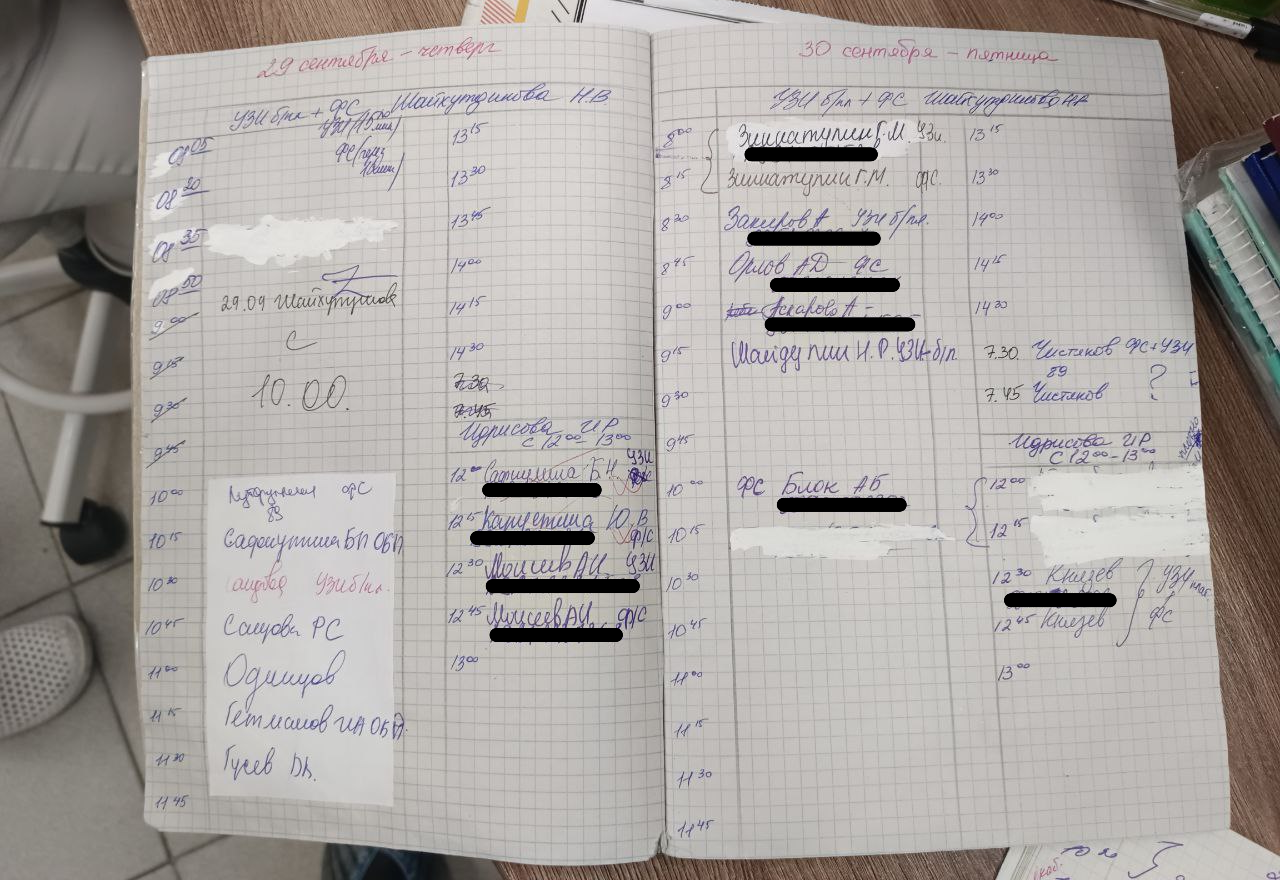
\includegraphics[width=0.8\linewidth]{Пример заполненной тетради на УЗИ+ФС. Чёрным закрашены номера телефонов.png}
            \caption{\centering Пример заполненной тетради на УЗИ+ФС. Чёрным закрашены номера телефонов}
            \label{fig:Тетрадь на УЗИ+ФС}
        \end{figure}

        Пациент, приходя в больницу, иду в регистратуру. Регистратор записывает его в тетрадь на конкретное время к конкретному врачу, вписывают его данные  -- ФИО, телефон, адрес и т.д. Далее в указанное время человек приходит к врачу.
        На первый взгляд схема проста и в ней сложно допустить ошибки, но если посмотреть внимательнее, то у неё много недостатков:

        \begin{itemize}[nolistsep]
            \item[--] Отсутствие синхронизации. Если пациент отменил запись, то изменение нужно сделать везде, где было упоминание о приёме.
            \item[--] Невозможность копирования. Каждый врач должен несколько раз в день сверяться с записью к нему, потому что актуальная копия только в регистратуре. При составлении отчётов также требуется переносить сведения о приёме. Вручную переписывать сотни строк.
            \item[--] Невозможность обработки. Если пациент пришёл на повторный приём, то предыдущую запись о нём нужно искать в разных архивных тетрадях, что сложно сделать человеку.
            \item[--] Дублирование информации. В РКИБ, по словам сотрудников, много регулярных пациентов. Если кто-то приходит каждый месяц, то в тетрадях он будет записан столько раз, сколько приходил. Редко когда у человека меняется, например, отчество или дата рождения. Эти данные записываются по нескольку раз, что не имеет практического смысла.
            \item[--] Невозможность качественного планирования расписания. У врачей часто меняется график работы, а в тетради строки фиксированы и ограничены. При любом изменении в графике нужно вручную найти конфликтующие пункты и изменить их.
            \item[--] Хранение неактуальной информации. Человек, поменявший место работы, навсегда в какой-то из тетрадей останется на прошлом.
        \end{itemize}

        Несмотря на недостатки, РКИБ использует этот способ. Всё из-за того, что он прост для понимания, доступен и к нему привыкли. Разработанная в результате система должна быть приближена к существующей, чтобы под неё не нужно было долго переучиваться.

    \subsubsection{1С:Медицина}

        <<1С:Медицина>> -- решение от компании 1С. Продуманное, сделанное профессионалами, проверенное временем. Пример интерфейса на Рисунке~\ref{fig:Интерфейс 1С:Медицина}~\cite{1cmedicine}. Это мог бы быть хороший вариант, но у него тоже есть недостатки:

        \begin{itemize}[nolistsep]
            \item[--] Отсутствие интеграции с существующими системами. Несмотря на то, что в РКИБ слабо информатизирована, часть процессов проходит в цифровой форме. Переход на 1С означает отказ от практически всего разработано ранее, либо дополнительные затраты на интеграцию.
            \item[--] Избыточность. Система нацелена на универсальность, поэтому в ней много функций, не нужных этой больнице, их можно было бы упростить. Сложность системы приводит к сложности её внедрения и обслуживания.
            \item[--] Цена и поддержка. Система стоит не малых денег, а поддержка будет требовать дополнительных вложений. При этом, если верить отзывам из открытых источников, поддержка и документация не всегда могут оперативно помочь.
        \end{itemize}

        \begin{figure}[h]
            \centering
            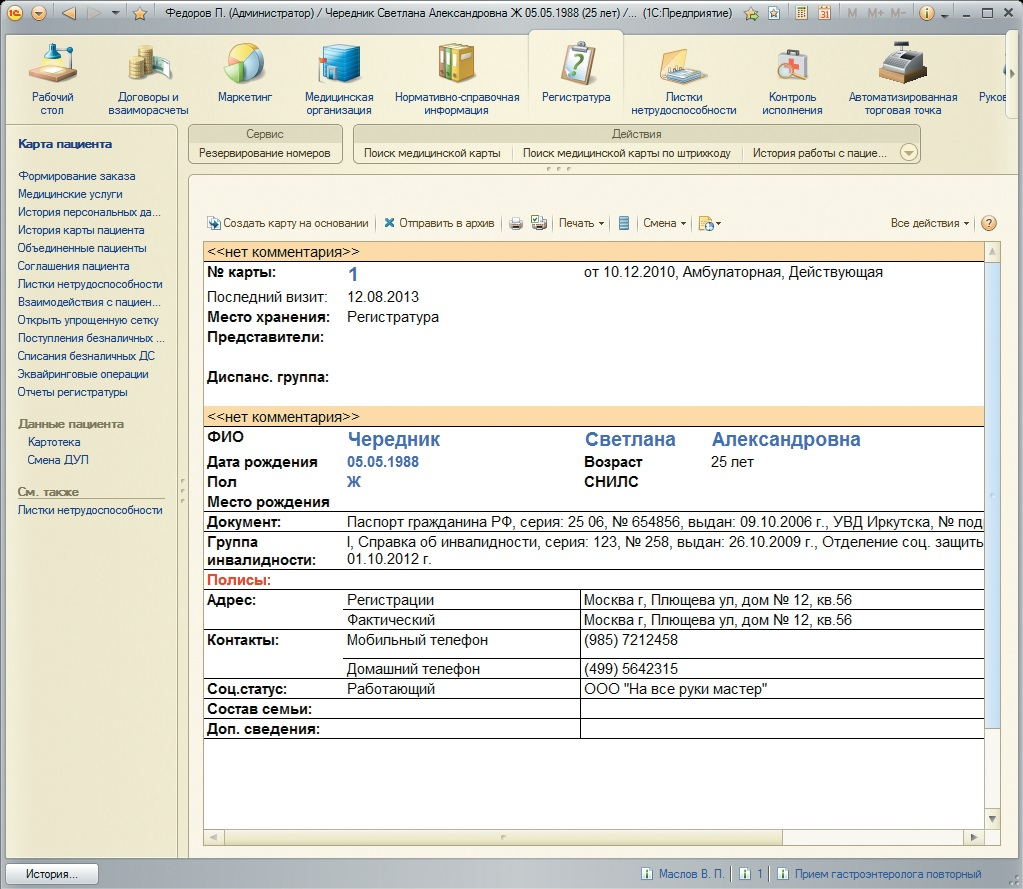
\includegraphics[width=0.6\linewidth]{Интерфейс 1С:Медицина.png}
            \caption{\centering Интерфейс 1С:Медицина}
            \label{fig:Интерфейс 1С:Медицина}
        \end{figure}
        
    \newpage

    \subsubsection{Другая предлагавшаяся система}

        Разрабатываемая система -- не первая, которую хотели внедрить в РКИБ. По словам сотрудников, им уже предлагали готовое решение. Проблема в том, что система не была приспособлена к использованию в этой больнице. Она подходила обычной поликлинике, но РКИБ слишком сильно от них отличается. Здесь нет привычных участков. Обслуживаются не только жители ближайших районов, но и, во том числе, других регионов. Это помешало внедрить её в РКИБ.

        Приспособленность к работе в условиях этой конкретной больницы -- важное условие для запуска системы.
        
    \subsubsection{Прочие системы}
    
        Существуют и другие системы записи, которые стоит упомянуть, но у них тоже есть существенные недостатки:
        
        \begin{itemize}[nolistsep]
            \item[--] СберЗдоровье. Партнёрство ограничено определёнными клиниками, отрицательные отзывы по качеству записи.
            \item[--] МедЭлемент. Наличие ошибок из-за технических неполадок. Не вся информация актуальная и точная.
            \item[--] Yell.ru. Ориентирована на поиск, а не на запись. Не специализирована на медицине. Возможна недостоверная и устаревшая информация.
        \end{itemize}

    \subsection{Техническое задание}\label{Техническое задание}

        В системе выделяются 4 роли:

        \begin{itemize}[nolistsep]
            \item[--] Пациент. Тот, кто имеет возможность попасть на приём.
            \item[--] Доктор. Принимает пациентов согласно своему расписанию, составляет своё расписание.
            \item[--] Регистратор. Записывает и подтверждает запись к врачу. Генерирует отчёты.
            \item[--] Администратор. Имеет доступ ко всем данным для их редактирования в случае возникновения проблем. Управляет редкоизменяемыми данными.
        \end{itemize}

        Каждая из них отличается требуемым функционалом. При этом каждый пользователь может иметь от 1 до 4 ролей, потому что врач, например, может записаться на приём к другому врачу. Рассмотрим функциональные требования к системе для каждой роли и нефункциональные требования, необходимые системе в целом.

    \subsubsection{Функциональные требования}\label{ТЗ. Функциональные требования}

        Как уже было сказано в пункте~\ref{Техническое задание}, в системе есть 4 роли. Диаграмма вариантов использования для этих ролей представлена на Рисунке~\ref{fig:Диаграмма вариантов использования}. Далее рассмотрим основные требования для каждой роли подробнее.

        \begin{figure}[h]
            \centering
            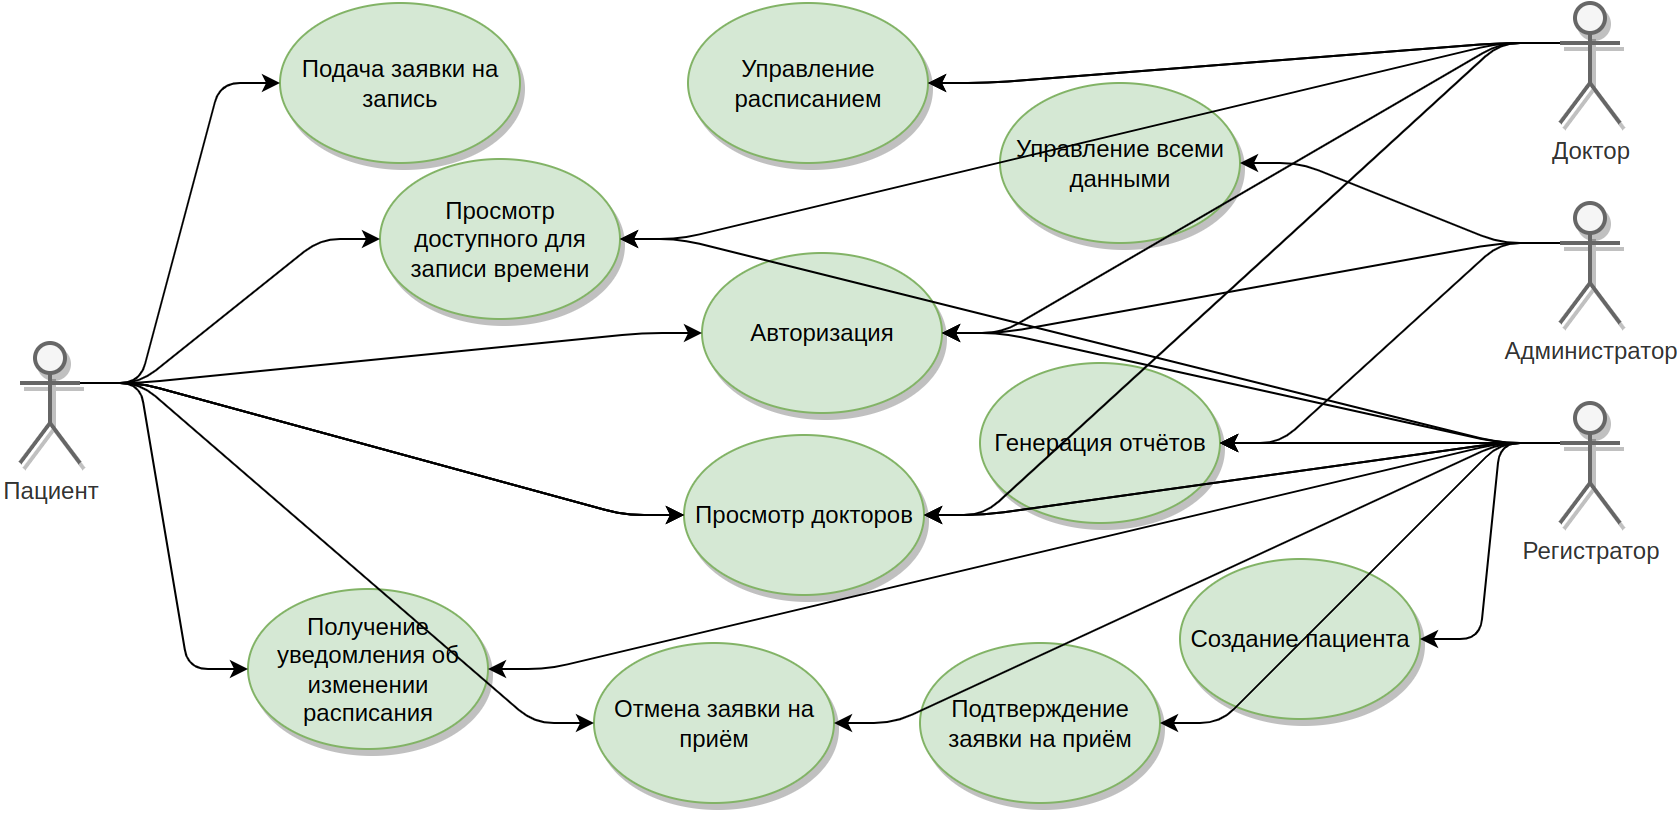
\includegraphics[width=0.9\linewidth]{Диаграмма вариантов использования.png}
            \caption{\centering Диаграмма вариантов использования}
            \label{fig:Диаграмма вариантов использования}
        \end{figure}

    \paragraph{Пациент}\label{ТЗ. Пациент}

    Функциональные требования для пациента:

    \begin{itemize}[nolistsep]
        \item[--] Авторизация. На первой странице приложения должна быть авторизация для пациентов. По логину и паролю пациент получает доступ к остальным функциям.
        \item[--] Просмотр докторов. Возможность узнать какие врачи работают в учреждении и какие у них специализации. Нужно для того, чтобы даже если врач болеет, то была информация о нём.
        \item[--] Просмотр времени для записи. Созданный врачом график записи должен отображаться для пользователя там же, где и <<Просмотр докторов>>, но при выборе конкретного доктора.
        \item[--] Заявка на запись. Выбрав время приёма, пользователь может нажать на кнопку <<Записаться>>. Заявка отправляется регистратору и время для записи закрывается. Одновременно активных заявок на приём у пациента может быть не более двух.
        \item[--] Отмена заявки на запись. Если по какой-то причине пациент не может попасть на приём, то на странице своих визитов он может нажать на кнопку <<Отменить запись>>. Сразу после этого время для приёма должно освободиться, а регистратору должно прийти об этом уведомление.
        \item[--] Просмотр своих визитов. Пациент может просмотреть информацию о своих прошлых визитах и о текущих записях с указанием информации об обращении.
    \end{itemize}

    \paragraph{Доктор}\label{ТЗ. Доктор}

    Функциональные требования для доктора:
        \begin{itemize}[nolistsep]
            \item[--] Авторизация. На первой странице приложения около панели входа должна быть кнопка для перехода на страницу входа как сотрудника. Отличается он возможностью указать роль в учреждении. После входа под конкретной ролью пользователя переносит на страницу этой роли.
            \item[--] Управление своим расписанием. Возможность создавать новые элементы своего расписания, отмечать недоступными те, в которые врач не сможет совершить приём.
            \item[--] Просмотр списка записанных к нему. Пациенты, которые записались на приём к врачу доступны для быстрого просмотра этому врачу. Если никто не записан на какое-то время, то об этом тоже должно быть написано. Если изменения в расписании касаются текущего рабочего дня, то об изменении в списке приёма дополнительно должно приходить уведомление.
            \item[--] Заполнение данных о приёме. Основная информация о приёме не затрагивает текущую систему, однако, должна быть возможность указания диагноза и комментария по приёму.
        \end{itemize}
        
    \newpage

    \paragraph{Регистратор}\label{ТЗ. Регистратор}

    Функциональные требования для регистратора:

    \begin{itemize}[nolistsep]
        \item[--] Авторизация. То же самое, что авторизация врача.
        \item[--] Создание/подтверждение записи пациента. Регистратор может самостоятельно записать пациента на приём если он, например, пришёл в учреждение. Особенно актуально для пожилых. Для этого регистратор указывает пациента и время приёма. Если же речь о подтверждении, то всё уже указано и требуется только его проверка.
        \item[--] Отмена записи на приём. По каким-либо причинам пациент может не прийти на приём. Если он сообщил об этом заранее, то есть до приёма есть время, то у регистратора есть возможность отменить запись.
    \end{itemize}

    \paragraph{Администратор}\label{ТЗ. Администратор}

    Функциональные требования для администратора:

    \begin{itemize}[nolistsep]
        \item[--] Авторизация. То же самое, что авторизация врача.
        \item[--] Управление всеми доступными данными системы. Должна быть страница для каждого элемента, который вообще можно изменять. Только администратор может менять список услуг, добавлять сотрудников, взаимодействовать со статусами.
    \end{itemize}

    \subsubsection{Нефункциональные требования}

    В этом разделе будут рассмотрены критерии, используемые для оценки работы системы -- характеристики производительности и атрибуты качества.

    \paragraph{Совместимость}\label{ТЗ. Интерфейс пользователя}

    Система должна корректно работать Chromium, Яндекс.Браузер, Edge версий, актуальных на начало 2023 года. Должна гарантироваться работа на экранах с разрешениями от 1024x768 до 1920x1440 для соотношения сторон 4:3, и с разрешениями 1280x720 до 1920x1080 для соотношения сторон 16:9. Указанные разрешения предполагают развёрнутость окно браузера на полный экран.

    \paragraph{Безопасность}\label{ТЗ. Безопасность}

    Использование системы должно происходить только через HTTPS. Пароли должны храниться в таком виде, чтобы из него было невозможно узнать изначальный пароль. Следовательно, не должно быть возможности восстановить пароль -- только сбросить и создать новый.

    \paragraph{Производительность}\label{ТЗ. Производительность}

    Система должна корректно работать при одновременном подключении как минимум 10 пользователей без значительного снижения производительности -- не более 10 секунд на запрос при условии стабильного подключения интернета 100Мбит/с.

    \newpage

    \section{Проектирование}\label{Проектирование}

    Разрабатываемая система -- клиент-серверное приложение. Общая схема клиент-серверного приложения представлена на Рисунке~\ref{fig:Схема клиент-серверного приложения}~\cite{webapi, cleanarch}.

    \begin{figure}[h]
        \centering
        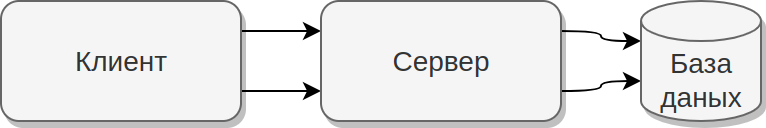
\includegraphics[width=0.6\linewidth]{Схема клиент-серверного приложения.png}
        \caption{\centering Общая схема клиент-серверного приложения}
        \label{fig:Схема клиент-серверного приложения}
    \end{figure}

    В этой главе будут спроектированы указанные части системы, а в главе~\ref{Реализация} -- выбраны инструменты и реализованы элементы приложения.

    \subsection{База данных}

    Для реализации системы потребуется база данных. Её цель -- упростить работу с данными для серверной логики. Появляется выбор -- использовать реляционную или нереляционную базу данных.

    Нереляционная база данных, с одной стороны, может повысить гибкость приложение, а с другой -- усложняет работу с данными. В разрабатываемой системе выигрыш от использования нереляционной базы данных минимален, потому что даже в тетрадях всё записывалось в виде простых таблиц. Реляционная база данных в этом случае подойдёт лучше -- с ней гораздо проще работать и они лучше подойдут для, например, поиска, потому что список полей фиксирован.

    Исходя из данных пункте~\ref{Текущее решение проблемы} можно выделить сущности базы данных~\cite{dbdesign}.

    \subsubsection{Основные таблицы}\label{Проектирование БД. Основные компоненты}

    Для создания схемы данных нужно проанализировать задачу: Система должна позволять связывать заявки людей на приём и время приёма. Получается, что основных компонентов должно быть 2: обращение и расписание. К этому же можно прийти из пункта~\ref{Текущее решение проблемы}: Для каждого обращения в тетради используется отдельная строка. Для расписания врачей тоже используется одна строка на одно время приёма. Простейшая возможная база данных -- состоящая из перенесённых из тетради строк в поля таблиц, получим:

    \begin{itemize}[nolistsep]
        \item[--] Обращение: Содержит данные пациента: ФИО, занятость, адрес для идентификации пациента. Дополнительно содержит направление и диагноз.
        \item[--] Расписание: Включает в себя ФИО врача, услугу, которую он оказывает, время и, опционально, данные об обратившемся человеке. Причём приём может быть сразу на 2 и более ячейки расписания. Связь <<Много к одному>>.
    \end{itemize}

    \subsubsection{Вспомогательные таблицы}\label{Проектирование БД. Вспомогательные компоненты}

    Рассмотрим данные, которые можно было бы вынести в отдельные таблицы, для удобства работы с ними. Дополнительные компоненты можем разделить на 2 категории:

    \begin{itemize}[nolistsep]
        \item[--] Отражающие существующую логику. Они напрямую взяты из тетрадей и понятны обычному человеку.
        \item[--] Упрощающие работу с данными. Нужны только для использования внутри системы.
    \end{itemize}

    \paragraph{Отражающие существующую логику}\label{Проектирование БД. Вспомогательные компоненты. Отражающие логику}

    \begin{itemize}[nolistsep]
        \item[--] Пациент: Хранит общую информацию о пациенте. Нужна для хранения информации о человеке, которая не обязательно должна быть у, например, врача. Так врачу не обязательно указывать свой личный телефон, если он не является одновременно пациентом.
        \item[--] Сотрудник: Нужна только для определения кто из людей какую роль занимает в учреждении.
        \item[--] Учреждение: Если пациент пришёл по направлению, то это направление должно было быть выдано каким-то учреждением.
        \item[--] Услуга: Медицинские учреждения предоставляют конкретный список услуг. Таблица фиксирует его.
    \end{itemize}

    \paragraph{Упрощающие работу с данными}\label{Проектирование БД. Вспомогательные компоненты. Упрощающие работу с данными}

    \begin{itemize}[nolistsep]
        \item[--] Человек: Сущность, объединяющая пациента и сотрудника. В обеих таблицах есть ФИО. К тому же аккаунт должен быть и у тех, и у тех. Более того, один и тот же человек может быть и пациентом, и сотрудником. Объединение нормализует данные.
        \item[--] Статус обращения: Вспомогательная таблица. Нужна для определения того, что делать с обращением. Например, чтобы отменённое обращение не показывалось в расписании врача.
        \item[--] Статус элемента расписания: Тоже вспомогательная таблица, но для других целей. Например, если врач заболел, то записанные к нему люди будут отдельно обработаны регистратором.
    \end{itemize}

    \subsubsection{Логическая схема данных}

    Исходя из пунктов \ref{Проектирование БД. Основные компоненты} и \ref{Проектирование БД. Вспомогательные компоненты} можно составить логическую схему данных, представленную на Рисунке~\ref{fig:Логическая схема данных}~\cite{dbdiag}.

    \begin{figure}[h]
        \centering
        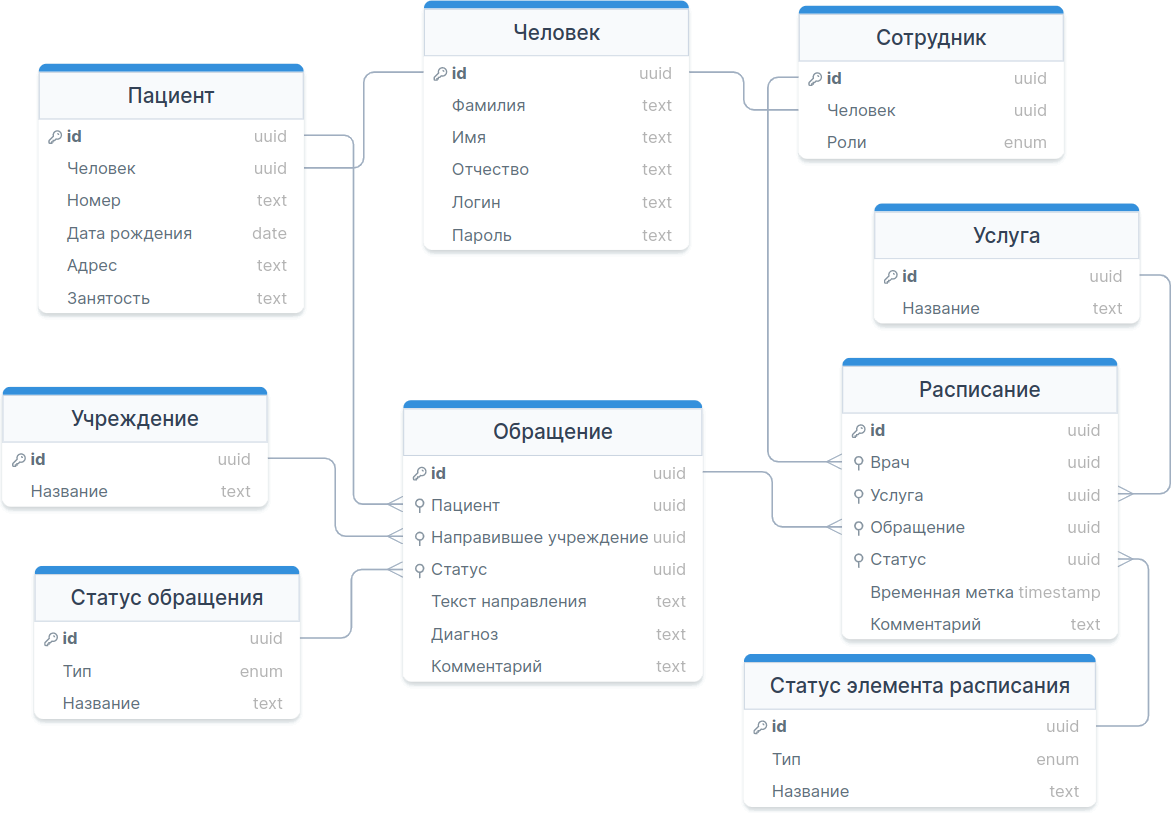
\includegraphics[width=0.9\linewidth]{Логическая схема данных.png}
        \caption{\centering Логическая схема данных разрабатываемой системы}
        \label{fig:Логическая схема данных}
    \end{figure}

    \newpage

    \subsection{Серверная часть}

    Клиентский код не должен напрямую обращаться к базе данных~\cite{baeldungbook, webapi, cleanarch}. Ему нужно промежуточное звено -- сервер. Передавать данные клиент и сервер должны заранее определённым способом -- API. Данные между клиентом и сервером передаются в формате, понятном обоим элементам. После преобразования данных в сущности, сервер работает напрямую с базой данных. Архитектура серверной части представлена на Рисунке~\ref{fig:Архитектура серверной части}

    \begin{figure}[h]
        \centering
        
\includegraphics[width=0.9\linewidth]{Архитектура серверной части.png}
        \caption{\centering Общая архитектура серверной части}
        \label{fig:Архитектура серверной части}
    \end{figure}
    
    \vspace{-2em}

    \subsubsection{Выбор вида API}\label{Выбор вида API}

    В зависимости от потребностей системы можно использовать разные виды API. Сравнение популярных видов API представлено в Таблице~\ref{tab:Популярные виды API}.

    \begin{xltabular}{\textwidth} { |
            >{\hsize=0.16\hsize} X |
            >{\hsize=0.44\hsize} X |
            >{\hsize=0.44\hsize} X | }
        \caption{\centering Популярные виды API}
        \label{tab:Популярные виды API} \\
            
        \hline
        Название
        & Плюсы
        & Минусы \\
        \hline
        REST
        & -- Универсальность \newline -- Поддержка CRUD \newline -- Легко масштабируется
        & -- Нет строгого стандарта \newline -- Падение производительности от количества запросов \\
        \hline
        SOAP
        & -- Безопасность \newline -- Поддержка транзакций \newline -- Строгий стандарт
        & -- Избыточность данных \newline -- Сложность использования и настройки \\
        \hline
        GraphQL
        & -- Нет избыточных данных \newline -- Возможность сложных запросов \newline -- Сильная типизация
        & -- Сложность разработки \newline -- Сложное масштабирование \newline -- Перегрузка из-за сложности запросов \\
        \hline
        gRPC
        & -- Быстрое выполнение \newline -- Сильная типизация
        & -- Сложность в настройке и использовании \\
        \hline
        JSON-RPC и XML-RPC
        & -- Простота использования и разработки \newline -- Лёгкость интеграции
        & -- Нет поддержки HTTP-методов \newline -- Трудное масштабирования \\
        \hline
    \end{xltabular}
    
    \newpage

    Для разработки был выбран REST. Его минусы в рамках проекта незначительны: в системе не будет большого количества запросов, а отсутствие строгого стандарта всего лишь делает его принципы рекомендациями. При этом REST удовлетворяет всем потребностям приложения -- поддержка HTTP-методов, отсутствие сохранения состояния, а также ранее использовался автором для своих проектов.

    \subsubsection{Авторизация}
    
    Авторизация -- важный элемент безопасности системы. Есть разные подходы к её организации и для выбора нужно учитывать потребности системы и технологии, например, выбранный в пункте~\ref{Выбор вида API} тип API.

    \begin{xltabular}{\textwidth} { |
            >{\hsize=0.20\hsize} X |
            >{\hsize=0.40\hsize} X |
            >{\hsize=0.40\hsize} X | }
        \caption{\centering Популярные виды API}
        \label{tab:Авторизация} \\
            
        \hline
        Название & Плюсы & Минусы \\
        \hline
        Basic Auth
        & -- Хорошо работает с HTTPS \newline -- Не требует сессий \newline -- Прост в реализации
        & -- Нет средств управления сессиями \newline -- Передача данных в незашифрованном виде \\
        \hline
        Digest Auth
        & -- Безопасность из-за хеширования для передачи данных
        & -- Сложность реализации \newline -- Нет управления сессиями \\
        \hline
        Token-based Auth \newline (JWT, OAuth)
        & -- Есть управление сессиями \newline -- Передача метаданных
        & -- Сложная реализация и управление токенами \newline -- Проблемы при больших объёмах данных \\
        \hline
        Session-based Auth
        & -- Управление сессиями \newline -- Сервер контролирует данные сессии
        & -- Хранение и управление данными сессии \newline -- Плохо масштабируется \\
        \hline
    \end{xltabular}

    Для данного проекта была выбрана Basic Auth, потому что он прост в реализации. Его проблема безопасности решается использованием HTTPS и он хорошо подходит для проектов небольшого масштаба.

    Заголовок авторизации -- специальная строка, передающаяся вместе с запросом. Выглядеть строка должна так: <<Authorization: Basic *токен*>>, где *токен* -- Это зашифрованная с помощью Base64 строка вида <<*логин*:*пароль*>>~\cite{baeldungbook}. При запуске приложения создаётся аккаунт по умолчанию, поэтому для всех методов, кроме установки пароля, потребуется авторизация.

    \subsubsection{Методы API}

    Каждый запрос на сервер в разрабатываемой системе характеризуется несколькими параметрами~\cite{baeldungbook}:

    \begin{itemize}[nolistsep]
        \item[--] URL
        \item[--] Метод HTTP
        \item[--] Заголовок авторизации
        \item[--] Параметры в теле запроса, либо в URL
    \end{itemize}

    Зная эти данные мы можем дать нужный ответ. Теперь нужно определить -- кто к каким конечным точкам должен иметь доступ. Для этого нужно составлять таблицы с указанием приведённых выше параметров.

    Хорошей практикой считается разделение версий API и выделение его в URL~\cite{baeldungbook}. Поэтому перед каждой конечной точкой в реальных запросах к API дополнительно используется /api/v1, если не сказано иное. Спроектированные методы API представлены в Таблице~\ref{tab:Методы API}.
    
    Можно видеть разделение конечных точек в зависимости от ресурса, который они предоставляют. Разные конечные точки поддерживают разные HTTP методы из-за различий в их функциях.
    
    \newpage

    \begin{xltabular}{\textwidth} { |
        >{\hsize=0.25\hsize} X |
        >{\hsize=0.20\hsize} X |
        >{\hsize=0.55\hsize} X | }
        \caption{\centering Методы API}
        \label{tab:Методы API} \\

        \hline
        URL 
        & HTTP метод 
        & Краткое описание \\

        \hline
        /people/\{id\}
        & GET, PUT, DELETE
        & Получение, изменение, удаление общих данных о человеке \\

        \hline
        /people/me
        & PUT, GET
        & Получение, изменение данных о себе \\

        \hline
        /people
        & POST, GET
        & Получение списка всех пользователей \\

        \hline
        /patients/\{id\}
        & GET, PUT, DELETE
        & Получение, изменение, удаление пациента \\

        \hline
        /patients
        & POST, GET
        & Получение списка всех пациентов \\

        \hline
        /employees/\{id\}
        & GET, PUT, DELETE
        & Получение, изменение, удаление сотрудника \\

        \hline
        /employees
        & POST, GET
        & Получение списка всех сотрудников \\

        \hline
        /institutions/\{id\}
        & GET, PUT, DELETE
        & Получение, изменение, удаление учреждения  \\

        \hline
        /institutions
        & POST, GET
        & Получение списка всех учреждений \\

        \hline
        /appointments/\{id\}
        & GET, PUT, DELETE
        & Получение, изменение, удаление обращения \\

        \hline
        /appointments
        & POST, GET
        & Получение списка всех обращений \\

        \hline
        /schedules/\{id\}
        & GET, PUT, DELETE
        & Получение, изменение, удаление элемента графика \\

        \hline
        /schedules
        & POST, GET
        & Получение списка всех элементов графика \\

        \hline
    \end{xltabular}

    Отдельно стоит выделить таблицы, к которым должен иметь доступ только администратор. Это такие таблицы, которые меняются очень редко и их изменение сильно влияет на всю систему. Например, изменение в таблице <<Услуги>>. Перечень запросов, доступных только Администратору представлен в Таблице~\ref{tab:Методы API только для Администатора}.
    
    \newpage

    \begin{xltabular}{\textwidth} { |
        >{\hsize=0.34\hsize} X |
        >{\hsize=0.18\hsize} X |
        >{\hsize=0.47\hsize} X | }
        \caption{\centering Методы API только для Администратора}
        \label{tab:Методы API только для Администатора} \\

        \hline
        URL
        & HTTP метод
        & Краткое описание \\

        \hline
        /procedures/\{id\}
        & GET, PUT, DELETE
        & Получение, изменение, удаление услуги \\

        \hline
        /procedures
        & POST, GET
        & Добавление услуги, получение всех услуг \\

        \hline
        /appointmentStatuses/\{id\}
        & GET, PUT, DELETE
        & Получение, изменение, удаление статуса обращения \\

        \hline
        /appointmentStatuses
        & POST, GET
        & Добавление статуса обращения, получение всех статусов обращений \\

        \hline
        /scheduleStatuses/\{id\}
        & GET, PUT, DELETE
        & Получение, изменение, удаление статуса элемента графика \\

        \hline
        /scheduleStatuses
        & POST, GET
        & Добавление статуса элемента графика, получение всех статусов элементов графика \\

        \hline
    \end{xltabular}

    \subsubsection{Обработка ошибок}\label{Проектирование сервера. Обработка ошибок}

    Обработку ошибок можно разделить на 2 больших пункта:

    \begin{itemize}[nolistsep]
        \item[--] На стороне сервера. Рассматривается в этом пункте ниже
        \item[--] На стороне клиента. Будет рассматриваться в пункте~\ref{Проектирование клиента. Обработка ошибок}
    \end{itemize}

    \paragraph{Обработка ошибок базы данных}

    Отдельно выделяются ошибки, связанные с базой данных. Это такие ошибки, которые может быть сложно, либо затратно обнаружить и обработать. Это связано с тем, что база данных -- отдельная часть системы, с которой взаимодействует сервер. Есть несколько основных моментов, которые стоит затронуть:

    \begin{itemize}[nolistsep]
        \item[--] Транзакционность. База данных хранит данные -- это её основная задача. Контроль корректности вводимых данных на её стороне возможен либо частичный (например, уникальность полей), либо очень затратен в создании и поддержке (триггеры). Если данные записались в базу данных, то может быть проблемой удалить их. Особенно это актуально при одновременном создании множества объектов, когда может выполниться только часть запросов. В таких случаях помогает транзакционность, то есть возможность отменить все изменения в рамках связанных запросов. В рамках разрабатываемой системы необходимо учитывать это на стороне сервера.
        \item[--] Определение конкретного места ошибки. Стандартные ошибки, выдаваемые базой данных, не всегда информативны для пользователя, а иногда и для администратора. Так, например, нарушение связи один к одному, либо конфликт из-за уникальности -- разные ошибки и их нужно по-разному идентифицировать.
    \end{itemize}

    \paragraph{Коды ошибок}\label{Проектирование сервера. Коды ошибок}

    Сопоставление каждой возможной ошибке конкретного кода может значительно ускорить процесс её обработки. Невозможно заранее знать все возможные причины ошибок -- тогда бы их просто не было. Но вполне осуществимо выявление части программы, в которой произошла ошибка. Например, есть код, отвечающий за чтение Person из базы данных. Если мы пометим эту часть кода как вызывающую ошибку с кодом drp-01, то при её возникновении заранее будет известно её расположение. Это не отменяет вспомогательных сообщений и логирования -- лишь помогает им. Список определённых кодов ошибок достаточно большой, их список приведён в Приложении~1.

    \paragraph{Единый формат ошибок}\label{Единый формат ошибок}

    Стандартные форматы ошибок могут отличаться от фреймворка к фреймворку, что уменьшает гибкость приложения. Дополнительно, не каждый формат ошибок подходит для каждого приложения -- в некоторых много избыточной информации, в некоторых её недостаточно. Хорошей практикой является написание своих формат ошибок~\cite{httpadderrors}, поэтому для приложения был разработан формат ошибок, использующий JSON. Представлен на Листинге~\ref{errformat}.
    
    \newpage
    
    \begin{lstlisting}[label=errformat,caption=Формат ошибок]
    {
        httpCode: "",
        errors: [
            {
                code: "",
                message: "",
                details: ""
            },
            ...
        ]
    }
    \end{lstlisting}

    Далее по частям разобраны части приведённого формата ошибок.

    \begin{itemize}[nolistsep]
        \item[--] httpCode. У протокола http есть перечень поддерживаемых кодов состояния~\cite{httpstatus}. Например, коды 2XX -- коды успешного выполнения запроса, 4XX -- ошибки клиента, 5XX -- ошибки сервера. Это общепринятые заданные стандартом коды. Здесь потребуются только коды, отвечающие за ошибки. Явное указание кода в ответе упрощает работу с ошибкой при отладке.
        \item[--] errors. Массив ошибок. Перечень того, что сервер в процессе обработки запроса посчитал некорректным. Стоит отметить, что перечисляются не все ошибки, а лишь те, до которых сервер обработал данные. Несколько элементов может быть указано только если ошибки одного типа, например, все касаются валидации полей.
        \begin{itemize}[nolistsep]
            \item[--] code. Внутренний код ошибки системы, определённый в пункте~\ref{Проектирование сервера. Коды ошибок}.
            \item[--] message. Написанное доступным простому пользователю языком сообщение об ошибке, выводимое на экран.
            \item[--] details. Более развёрнутое сообщение об ошибке, содержащее максимум данных для отладки. Опциональное поле.
        \end{itemize}
    \end{itemize}

    Использование этого стандарта гарантирует, что даже при переходе на другой фреймворк одной из частей приложения, изменения коснутся только её. Иначе в зависимости от фреймворка нужно было бы либо приводить вид одного к другому, либо переделывать и клиентскую, и серверную части~\cite{httpstatus}.

    \newpage

    \subsection{Клиентская часть}

    Клиентская часть завершает список необходимых компонентов для клиент-серверного приложения. Это та часть, которую пользователь видит на экране. Сюда, по большей части, относится графический интерфейс и работа с ним. Сюда же входит работа с API сервера: формирование запросов, обработка ответов~\cite{baeldungbook, webapi}.

    \subsubsection{Архитектура клиентского приложения}

    Для разработки понадобятся различные компоненты, такие как диалоговые окна, кнопки, элементы для поиска элементов~\cite{vuejs}. Рассмотрим, какие компоненты нужны для работы системы:

    Поля ввода. Может показаться, что это один компонент, но для удобной работы нужно детализировать его для разных нужд:

    \begin{itemize}[nolistsep]
        \item[--] Обычные поля, не требующие особого подхода. Например, комментарий к обращению может быть написан в свободной форме.
        \item[--] Пароль. Требует сокрытия вводимых данных.
        \item[--] Поля со строго определённой структурой. Необходимы для, например, наглядного ввода номера телефона
    \end{itemize}

    Кроме того, большинство полей в базе данных приложения требуют гарантии заполненности. Так, услуга не имеет смысла без её названия. Нужна возможность визуальных подсказок для полей.

    Алерты. Компоненты, информирующие пользователя о событиях. Когда на странице не могут загрузиться данные, либо произошла какая-то ещё ошибка, то нужно об этом сказать пользователю. Для этого хорошо подходит отдельный компонент.

    Выпадающие списки. Заменяют поля ввода, когда список его значений заранее известен и достаточно мал.

    Диалоговые окна. Это элементы, появляющиеся поверх основной страницы и служащие для совершения какого-то фиксированного действия. Например, отправка запроса на создание элемента или выбор элемента из множества на основе фильтров. В разделе~\ref{Техническое задание} упоминалось, что в системе будет Администратор. Он должен иметь возможность редактировать все записи в базе данных. Для этого ему потребуется диалоговое окно на каждую из сущностей. Они же будут использоваться и для остальных ролей в случаях, когда доступ к сущностям есть.

    \subsubsection{Проектирование интерфейса пользователя}
    
    \paragraph{Переходы между страницами}

    В пункте~\ref{Техническое задание} выделено 4 роли: Пациент, доктор, регистратор, администратор. У каждого из них, в соответствии с пунктами~\ref{ТЗ. Пациент}~--~\ref{ТЗ. Администратор} в системе свои возможности. Для этого необходимо разграничение интерфейса. Роли с указанием доступных им страниц и переходов между ними показаны на Рисунке~\ref{fig:Диаграмма переходов между страницами}. Сами страницы будут представлены в пункте~\ref{Реализация. Клиентская часть. Пользовательский интерфейс}.
    
    \begin{figure}[h]
        \centering
        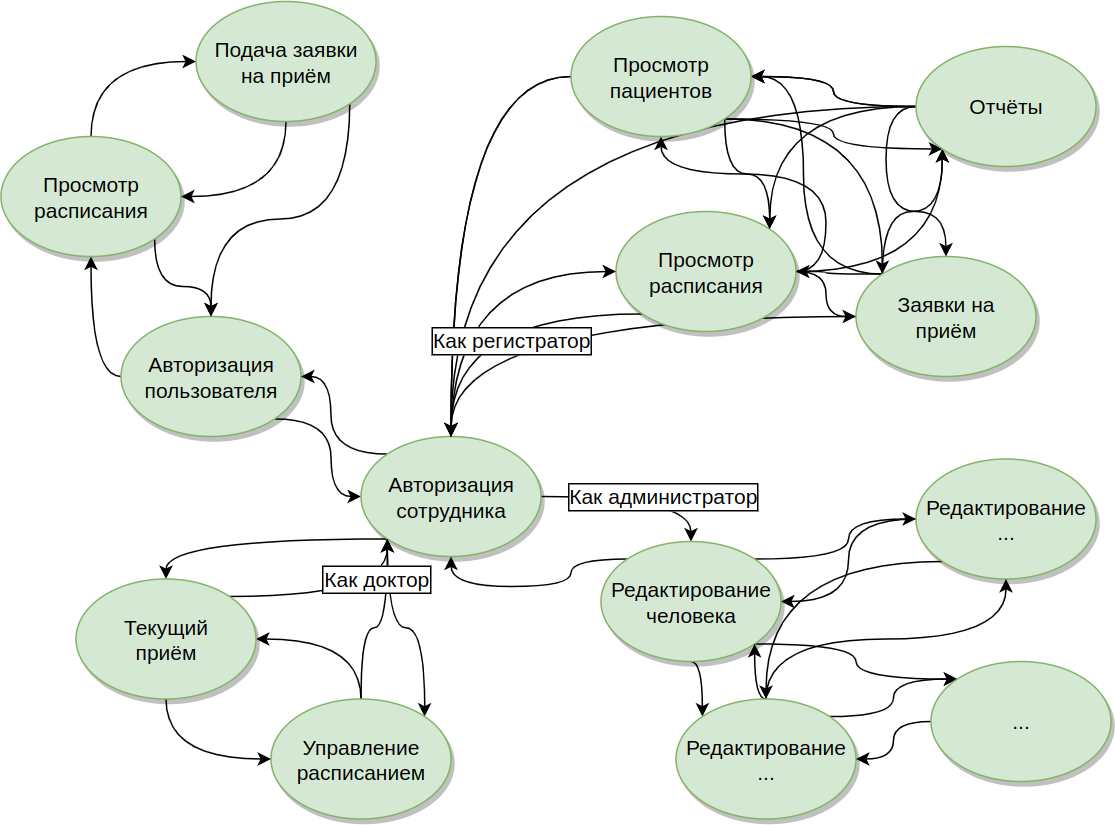
\includegraphics[width=0.9\linewidth]{Диаграмма переходов между страницами.png}
        \caption{\centering Диаграмма переходов между страницами}
        \label{fig:Диаграмма переходов между страницами}
    \end{figure}
    
    \newpage
    
    \paragraph{Цветовая палитра}
    
    Забегая вперёд -- для реализации будет использоваться Vue с библиотекой компонентов Vuetify. Эти инструменты нацелены на Material Design~\cite{vuetify} и используют соответствующую цветовую палитру, изображённую на Рисунке~\ref{fig:colorscheme}. В системе используются цвета <<Green>>, <<Red>>, <<Indigo>>, <<Grey>> и обычный белый цвет (\#FFFFFF) для фона и некоторого теста.
    
    \begin{figure}[h]
        \centering
        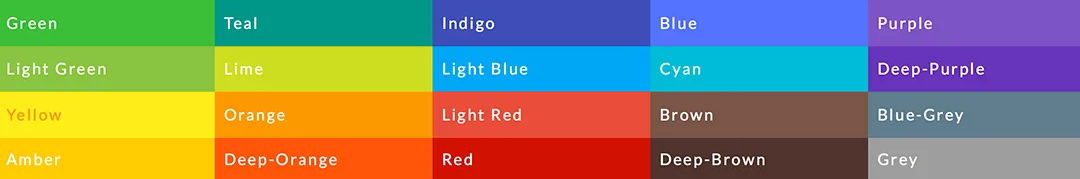
\includegraphics[width=0.8\linewidth]{Цветовая палитра.png}
        \caption{\centering Цветовая палитра}
        \label{fig:colorscheme}
    \end{figure}
    
    \vspace{-1em}

    \subsubsection{Обработка ошибок}\label{Проектирование клиента. Обработка ошибок}

    Важная часть разработки клиентского приложения -- правильная обработка ошибок. Она помогает предотвратить прерывание работы приложения, выявить и устранить причину ошибок. Продуманная система обработки ошибок важна для стабильности приложения~\cite{vuejs}.

    Существуют разные виды ошибок, которые должно обрабатывать клиентская сторона, например:

    \begin{itemize}[nolistsep]
        \item[--] Обработка ошибок на уровне приложения
        \item[--] Ошибки, генерируемые сервером. Например, запрос недоступного пользователю ресурса
        \item[--] Некорректный ввод пользователя. Частично относится к прошлому пункту, но выделение позволяет сделать интерфейс удобнее
        \item[--] Недоступность сервера
    \end{itemize}

    Подробнее рассмотрим важные элементы обработки ошибок

    \paragraph{Валидация данных}\label{Проектирование клиента. Валидация данных}

    Для предотвращения ошибок, связанных с неверными данными, в приложении необходимы механизмы проверки ввода -- валидации. Это включает валидацию свойств компонентов, использование библиотек для валидации форм и других пользовательских данных посредством специальных заранее определённых правил~\cite{baeldungbook}.

    \paragraph{Логирование ошибок}

    Для упрощения отладки и мониторинга работы приложения необходимо использовать систему логирования ошибок~\cite{cleancode}. Важно одновременно и уведомлять пользователя об ошибках, и выводит подробные данные о них, поскольку это разные уровни взаимодействия. Первые события рассчитаны больше на пояснение того, что случилось, в понятной простому человеку форме, а вторые -- на то, что их будет разбирать специалист, для чего нужно сохранять больше информации.

    \paragraph{Обработка ошибок в пользовательском интерфейсе}

    Информативные сообщения об ошибках и уведомлениях в пользовательском интерфейсе улучшают пользовательский опыт. Основная реализация -- всплывающие подсказки и уведомления. Стоит затронуть и необходимость визуального выделения ошибок, касающихся валидаций данных из пункта~\ref{Проектирование клиента. Валидация данных}.

    \newpage

    \section{Реализация}\label{Реализация}

    После анализа предметной области и проектирования остаётся последний большой шаг -- реализация. Потребуется написать код всех частей системы, сделать так, чтобы они работали вместе и без ошибок. Важным аспектом является тестирование, которое должно проводиться на протяжении всей разработки системы и даже до неё -- подход TDD <<Разработка через тестирование>>~\cite{tdd}.

    \subsection{Выбор технологий}\label{Реализация. Выбор}

    Выбор инструментов реализации проводится параллельно с проектированием. Это начальный этап разработки, который может определять структуру системы. В пункте~\ref{Проектирование} указано, что частей системы 3: база данный, серверная и клиентские части. Рассмотрим реализацию каждой из них ниже. Отдельно стоит упомянуть технологию изоляции приложений, которую будет использовать каждая из частей -- Docker~\cite{dockerdoc}.

    \subsubsection{Развёртывание}\label{Реализация. Выбор. Докер}

    Docker -- специальное средство, позволяющее создавать изолированное окружение для приложения. Это обеспечивает одинаковую работу на любом устройстве, где приложение будет запущено~\cite{dockerdoc}. Основной файл конфигурации -- Dockerfile. Он содержит необходимые настройки для работы приложения. Пример такого файла конфигурации для серверной части приведён на Листинге~\ref{dockerfileback}.

    \begin{lstlisting}[label=dockerfileback,caption=Пример Dockerfile для бекенда]
    FROM openjdk:17
    ARG JAR_FILE=build/libs/*.jar
    RUN mkdir /opt/rkib-appointment-backend
    COPY ${JAR_FILE} /opt/rkib-appointment-backend/rkib-appointment-backend.jar
    ENTRYPOINT ["java","-jar","/opt/rkib-appointment-backend/rkib-appointment-backend.jar"]
    \end{lstlisting}

    С помощью этого файла конфигурации уже можно запускать приложение в изолированной среде. Есть ещё один инструмент, помогающий в работе с контейнерами -- docker-compose~\cite{dockerdoc}. Он помогает в организации нескольких контейнеров, если они должны быть запущены вместе. Также позволяет писать удобочитаемый файл конфигурации. Пример такого файла конфигурации -- docker-compose.yml представлен на Листинге~\ref{docker-composeyml}. Теперь для полного разворачивания приложения достаточно одной команды в директории с этим файлом -- <<docker-compose~up~-d>>.

    \begin{lstlisting}[label=docker-composeyml,caption=Пример файла конфигурации docker-compose.yml]
    version: "3.9"
    services:
      rkib-appointment-backend:
      image: zalimannard/rkib-appointment-backend:latest
        container_name: rkib-appointment-backend
        ports:
          - 8116:8116
        depends_on:
          - rkib-appointment-db
        environment:
          - DB_URL=*database url*
          - DB_USER=*database user username*
          - DB_PASSWORD=*database user password*
          - DDL_BEHAVIOUR=*what happens to the database*
          - ADMIN_USERNAME=*back's admin username*
          - ADMIN_PASSWORD=*back's admin password*
        restart: unless-stopped
    \end{lstlisting}

    \subsubsection{База данных}\label{Реализация. Выбор. База данных}

    Изначальное условие для системы было -- использование СУБД Oracle~\cite{oracle}. Если разработанная система будет внедряться, то чтобы не было конфликтов в базе данных. Потому что разные СУБД имеют разные ограничения на имена, например, на длину и зарезервированные слова. Забегая вперёд -- вся работа с базой данных будет через спецификацию JPA, то есть смена СУБД почти не потребует затрат.

    \newpage

    \subsubsection{Серверная часть}\label{Реализация. Выбор. Серверная часть}

    При выборе технологического стека для серверной части важно учитывать такие требования, как производительность, стабильность, безопасность, масштабируемость. Сравнение основных стеков представлено в Таблице~\ref{tab:Сравнение технологических стеков для серверной части}~\cite{backstack}.

    \begin{xltabular}{\textwidth} { |
        >{\hsize=0.30\hsize} X |
        >{\hsize=0.70\hsize} X | }
        \caption{\centering Сравнение технологических стеков для серверной части}
        \label{tab:Сравнение технологических стеков для серверной части} \\

        \hline
        Состав стека
        & Особенности \\

        \hline
        Java + Spring
        & -- Высокая производительность и скорость выполнения \newline -- Хорошая интеграция с Oracle Database \newline -- Богатый набор библиотек для различных задач \newline -- Строгая статическая типизация для повышения надежности кода \newline -- Многопоточная модель, подходящая для CPU-интенсивных операций и масштабируемых систем \\

        \hline
        Python + Django
        & -- Скорость разработки \newline -- Много функций <<из коробки>> \newline -- Динамическая типизация \newline -- Меньшая производительность по сравнению с Java \newline -- Интеграция с Oracle может быть менее гибкой \\

        \hline
        JavaScript + Node.js
        & -- JavaScript на сервере и клиенте, упрощает разработку \newline -- Однопоточная модель с асинхронной I/O, эффективной для обработки большого количества коротких запросов \newline -- Низкая производительность для CPU-интенсивных операций по сравнению с Java \newline -- Динамическая типизация и возможные проблемы безопасности \\

        \hline
    \end{xltabular}
    
    \newpage

    Для представления API в удобном виде будет использоваться Swagger. Он обеспечивает автоматическую генерацию документации по API с возможностью запуска команд из него же. Удобный инструмент для тестирования в процессе разработки.

    Для автотестов будет использоваться RestAssured для запросов на сервер~\cite{restassured}, JUnit5 для организации тестов, AssertJ для повышения читаемости тестов и Allure для визуализации результатов тестирования. Они помогают быстро находить проблемы в коде и увеличивают эффективность рефакторинга.

    Lombok -- библиотека для Java, позволяющая сосредотачиваться на написании бизнес-логики, а не на написании шаблонного кода~\cite{lombok}. Так, практически пропадает необходимость написания геттеров, сеттеров, конструкторов и прочих компонентов. Код становится более чистым и легко поддерживаемым.

    \subsubsection{Клиентская часть}\label{Реализация. Выбор. Клиентская часть}

    У клиентский части приложения большое количество нюансов, которые нужно учесть. Они связаны с тем, что этот код будет выполняться на разных компьютерах и нужно обеспечить корректную работу на них.

    Основной язык разработки -- JavaScript. TypeScript -- разработанный компанией Microsoft язык, расширяющий возможности TypeScript: обладает статической типизацией, поддержкой полноценных классов. К тому же он совместим с JavaScript. Он повышает читаемость кода, его повторное использование и скорость поиска ошибок.

    JavaScript отвечает за внутреннюю логику, за внешний вид отвечают HTML и CSS. Можно писать код используя только их, но такой подход хорош только для очень маленьких приложений. Так, работу на разных экранах придётся обеспечивать вручную. Как и следить за цветовой палитрой, стилями и анимацией. Гораздо удобнее использовать фреймворки, так как они представляют готовый набор стандартных элементов и логики. Сравнение трёх самых популярных фреймворков~\cite{comparejs}:

    \begin{itemize}[nolistsep]
        \item[--] React. Гибкий, с большим количеством библиотек, но для полноценной разработки именно потребуется использование сторонних библиотек, что может быть затруднением.
        \item[--] Angular. Большой фреймворк со всеми нужными компонентами из коробки, чёткая структура, но сложный для изучения и малопроизводительный.
        \item[--] Vue.js. Гибкий, самодостаточный фреймворк с возможностью интеграции со сторонними библиотеками. Прост в освоении, хорошая документация, но меньше материала по сравнению с другими.
    \end{itemize}

    На основании личного опыта работы с Vue.js, можно выбрать его как подходящий инструмент для разработки данной системы. С учётом масштаба приложения, встроенных инструментов Vue.js будет достаточно для эффективной реализации всех необходимых функций~\cite{vuejs}. Для тестирования пользовательского интерфейса будет использоваться Selenide~\cite{selenide} -- удобная обёртка для библиотеки автоматического тестирования Selenium. Для визуализации тестов будет использоваться Allure с расширением для Selenide. Используемая система сборки -- Vite~\cite{vite}.

    \subsection{База данных}\label{Реализация. База данных}

    Как уже было сказано в пункте~\ref{Реализация. Выбор. База данных}, база данных будет создана через JPA~\cite{springguide}. Это спецификация, обеспечивающая переносимость данных между реляционными базами данных для приложений на Java. В файле конфигурации указано, как поступать с базой данных при каждом запуске приложения. Это указано в файле конфигурации, описанном в пункте~\ref{Реализация. Выбор. Докер}. За это отвечает параметр {DDL\_BEHAVIOUR}. Если требуемая база данных отличается от существующей, то в существующую вносятся необходимые изменения.

    Таблицы и поля в базе данных создаются с помощью JPA, то есть объекту в базе данных соответствует объект в Java. Это позволяет работать с хранящимися данными так, будто они уже являются объектами в Java~\cite{baeldungbook}. Это уже часть пункта~\ref{Реализация. Серверная часть}, но его необходимо разобрать отдельно. Это некая прослойка между СУБД и сервером. Для примера возьмём сущность Patient, описанную как Пациент в логической схеме данных на Рисунке~\ref{fig:Логическая схема данных}. Код представлен в Листинге~\ref{jpapatient}. По порядку разберём написанное:

    Строки 1-2 -- аннотации JPA, отвечающие за создание таблицы в базе данных. @Entity говорит, что класс является объектом базы данных, @Table указывает конкретное название таблицы в базе данных.

    Строки 3-7 -- аннотации библиотеки Lombok. Создают геттеры и сеттеры (методы для доступа к полям), реализует шаблон строитель (позволяет гибко создавать объекты) и генерирует 2 конструктора -- с требуемыми параметрами и всеми. Это нужно для инъекции зависимости, используемой в Spring и для работы шаблона строитель. Дополнительно опущены методы .equals() и hashcode, который сравнивает 2 экземпляра одного класса по заданным параметрам. В этом случае -- сравнение по полю id, так как в базе данных гарантируется уникальность первичного ключа.

    Все остальные таблицы делаются по аналогии, схема данных представлена на Рисунке~\ref{fig:Логическая схема данных}.

    \begin{lstlisting}[label=jpapatient,caption=Пример реализации таблицы Patient через JPA]
    @Entity
    @Table(name = "patients")
    @Getter
    @Setter
    @Builder(toBuilder = true)
    @RequiredArgsConstructor
    @AllArgsConstructor
    public class Patient {
        @Id
        @GeneratedValue(strategy = GenerationType.UUID)
        @Column(name = "id")
        private String id;
        @OneToOne
        @JoinColumn(name = "person_id", referencedColumnName = "id", nullable = false)
        private Person person;
        @Column(name = "birthdate")
        LocalDate birthdate;
        @Column(name = "phoneNumber", nullable = false)
        private String phoneNumber;
        @Column(name = "address")
        private String address;
        @Column(name = "occupation")
        private String occupation;
    }
    \end{lstlisting}

    В строках 9-12 объявляется первичный ключ и его тип генерации -- UUID. Есть разные способы генерации первичного ключа -- по последовательности, автоувеличением значения, какой-либо строкой, либо можно написать вообще свою функцию генерации. Одно из изначальных ограничений системы -- использование строкового первичного ключа. UUID подходит под эту роль. Это способ генерации уникальной последовательности, из-за чего сложно угадать его соседние элементы, что более безопасно, чем другие способы. Распространённая практика делать поле id в каждой таблице.

    В сторках 13-15 указано, что таблицы Person и Patient связаны <<Один к одному>>, то есть одному пациенту соответствует один аккаунт. Содержится ссылка и то, что пациент гарантировано имеет аккаунт.

    Строки 16-17 содержат информацию о дате рождения. Дата всегда сложный элемент, потому что, например, часовой пояс не должен влиять на дату рождения. У даты рождения не должно быть времени вообще. LocalDate позволяет гибко работать с датой.

    Далее в строках 16-23 содержатся обычные текстовые поля, характерные для таблицы пациент. Указывается имя и то, что это обычное поле в базе данных.

    Компонент Patient полностью покрывает все нюансы базы данных в создаваемой системе. Все остальные таблицы делаются по аналогии с рассмотренной. При запуске приложения все таблицы автоматически создадутся и свяжутся. Всё это происходит через обычные запросы к базе данных, но автоматически, через обёртку JPA.

    \subsection{Серверная часть}\label{Реализация. Серверная часть}

    \subsubsection{Структура проекта}

    Для начала рассмотрим структуру файлов проекта серверной части, она представлена на Листинге~\ref{backendprojectstructure}. Два важных файла вынесены на самый верх структуры -- главный файл приложения RkibAppointmentBackendApplication, содержащий только метод main с запуском Spring.

    Пакет config содержит файлы конфигурации безопасности, он будет рассмотрен в пункте~\ref{Реализация. Сервер. Безопасность}. Validator содержит только файл с указанием шаблона для номера. Его использование будет продемонстрировано в пункте~\ref{Реализация. Сервер. Архитектура слоёв}.
    
    \newpage

    \begin{lstlisting}[label=backendprojectstructure,caption=Структура серверного приложения]
    RkibAppointmentBackendApplication.java
    schema/
        appointment/
            status/
        institution/
        person/
            employees/
            patient/
        procedures/
        schedule/
            status/
    config/
    exception/
    validator
    \end{lstlisting}

    Пакет exception содержит реализацию ошибок, спроектированных ранее в пункте~\ref{Единый формат ошибок}. Приложение может выдавать ошибки с кодами 400 -- неверный запрос, 401 -- неавторизованный запрос, 403 -- нет доступа, 404 -- не найдено, 409 -- конфликт. Причём ошибки 401 и 403 может генерировать сам Spring (конкретно -- Spring Security). Нужно перехватывать эти ошибки, это делается с помощью класса с аннотацией @ControllerAdvice, перехватывающим конкретные ошибки Spring Security, например, валидацию. Код части этого класса приведён на Листинге~\ref{validationadvice}.
    
    Указывается конкретный тип перехватываемой ошибки, далее формируется ошибка в заданном для системы формате и вместо стандартной ошибки Spring на запрос возвращается она.
    
    Основное приложение находится в schema -- описание сущностей и работы с ними. Разделение -- по логическим единицам, таким как Учреждение, Человек. При этом Пациент и Сотрудник вложены в пакет Человек, а статус вложен в то, статусом чего он является. В каждом из пакетов содержатся файле, которые соответствуют архитектуре слоёв, которая будет рассмотрена далее в пункте~\ref{Реализация. Сервер. Архитектура слоёв}.
    
    \newpage

    \begin{lstlisting}[label=validationadvice,caption=Класс-прехватчик ошибок Spring]
    @ControllerAdvice
    public class ValidationAdvice {
        @ResponseBody
        @ExceptionHandler(ConstraintViolationException.class)
        @ResponseStatus(HttpStatus.BAD_REQUEST)
        public ExceptionResponse onConstraintValidationException(
        ConstraintViolationException e
        ) {
            List<ExceptionMessage> errors = e.getConstraintViolations().stream().map(
            violation -> ExceptionMessage.builder()
            .message(violation.getMessage())
            .details(violation.getPropertyPath().toString()).build()
            ).toList();
            return ExceptionResponse.builder()
            .httpCode(HttpCodes.BAD_REQUEST.getCode())
            .errors(errors)
            .build();
        }
        ...
    }
    \end{lstlisting}

    \subsubsection{Архитектура слоёв}\label{Реализация. Сервер. Архитектура слоёв}

    Архитектура слоёв -- подход к проектированию, где функциональность разделяется на отдельные слои. Каждый слой изолирует свою логику~\cite{baeldungbook, springguide, cleanarch}. Архитектура сервера представлена на Рисунке~\ref{fig:Схема работы сервера}.

    \begin{figure}[h]
        \centering
        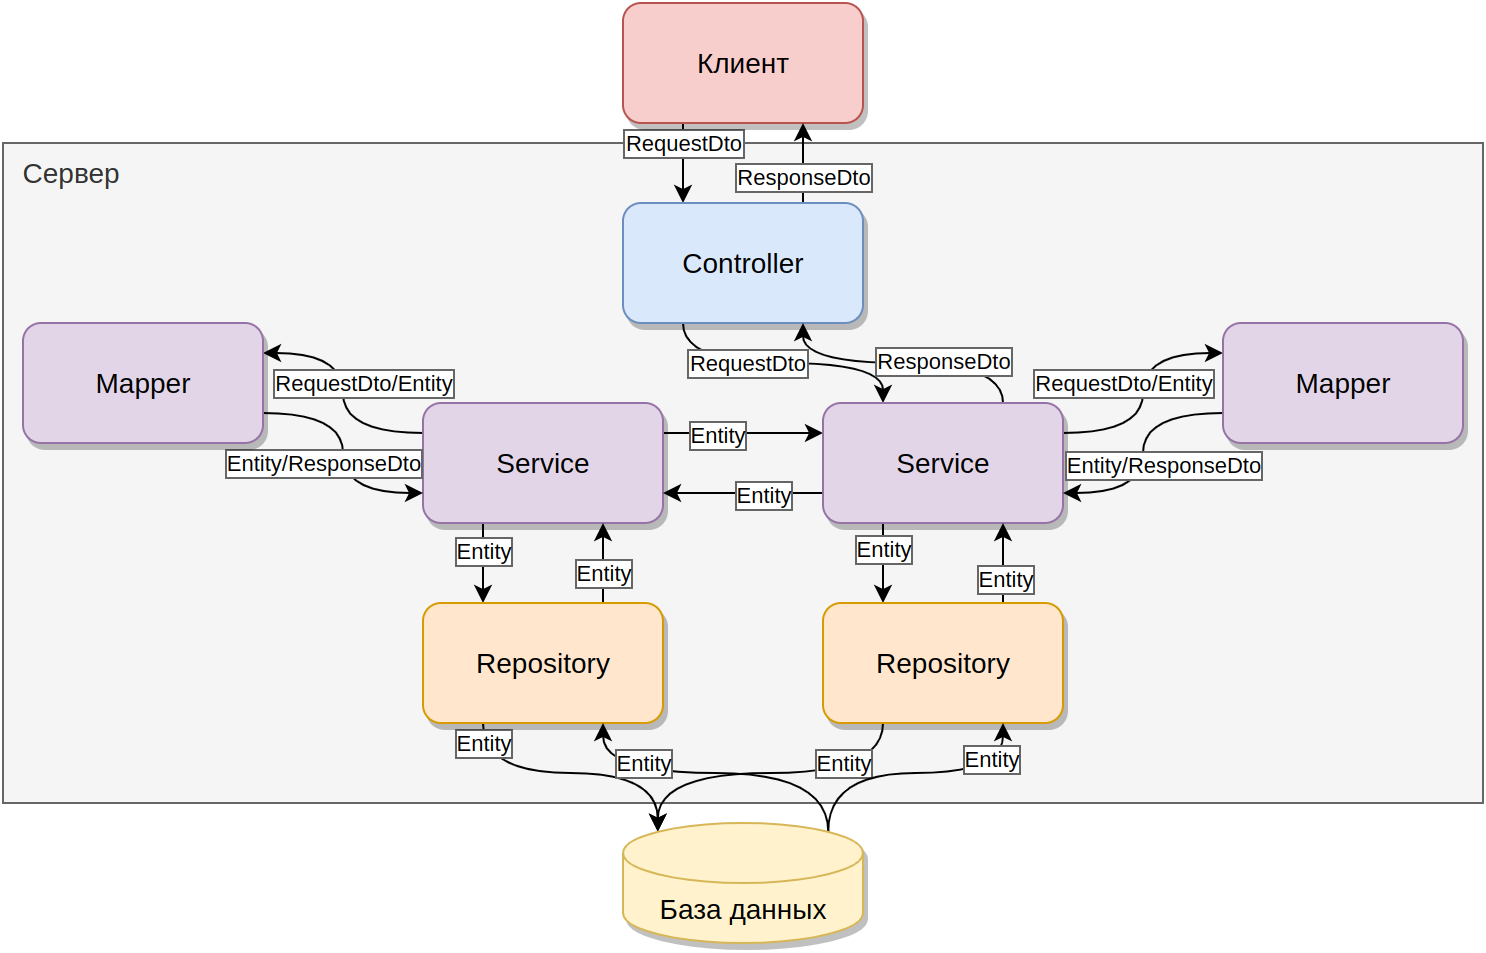
\includegraphics[width=0.9\linewidth]{Схема работы сервера.png}
        \caption{\centering Архитектура слоёв сервера}
        \label{fig:Схема работы сервера}
    \end{figure}

    Изображено разделение логики на слои представления (Controller), бизнес-логики (Service и вспомогательный для него Mapper), доступа к данным (Repository). Отображено, какими объектами они обмениваются. Далее рассмотрим каждый из компонентов подробнее. Один из компонентов -- Entity уже был рассмотрен в пункте~\ref{Реализация. Выбор. База данных}. Элемент <<Клиент>> соответствует схеме с Рисунка~\ref{fig:Схема работы клиента}, которая будет рассмотрена далее.

    \paragraph{DTO}\label{Реализация. Сервер. DTO}

    Клиент и сервер обмениваются данными через HTTP-запросы. В теле запросов передаётся информация в формате JSON, которая должна преобразовываться во внутренний объект сервера -- DTO (объект передачи данных) в Entity.

    Возникает проблема, когда запрос и ответ должны иметь разную структуру. Так, неразумно возвращать пароль пользователю. Можно его убирать перед отправкой, но надёжнее вообще не давать возможности отправить нежелательные данные. Также если в теле ответа нужно возвращать дополнительные данные, то им вовсе не обязательно быть в теле запроса. Поэтому DTO дополнительно разделяется на DTO для запросов и DTO для ответов~\cite{baeldungbook}. Сравнение этих двух типов DTO для  представлено в Таблице~\ref{tab:Сравнение объектов передачи данных для запроса и ответа}.
    
    Символом <<*>> отмечены отличающиеся элементы. Здесь это значит, что password не будет возвращён в ответе. При этом будет добавится id -- первичный ключ в базе данных, служащий идентификатором. С его помощью можно делать запросы конкретно с этим элементом. Далее появляются patient и employee. С обеими из таблиц Пациент и Сотрудник у таблицы Человек связь один к одному. Если человек является сотрудником, то для него будет дополнительно вложен объект такой, будто запросили информацию не просто о человеке, а о нём как сотруднике. Это уменьшает количество запросов и упрощает работу с данными~\cite{baeldungbook, webapi}.

    \begin{xltabular}{\textwidth} { |
        >{\hsize=0.50\hsize} X |
        >{\hsize=0.50\hsize} X | }
        \caption{\centering Сравнение объектов передачи данных сущности Person для запроса и ответа}
        \label{tab:Сравнение объектов передачи данных для запроса и ответа} \\

        \hline
        Тело запроса
        & Тело ответа \\

        \hline
        -- email \newline -- password * \newline -- lastName \newline -- firstName \newline -- patronymic
        & -- id * \newline -- email \newline -- lastName \newline -- firstName \newline -- patronymic \newline -- patient * \newline -- employee * \\

        \hline
    \end{xltabular}

    Оба типа DTO используются только для передачи данных между клиентом и сервером и при первой же возможности заменяются на внутренние объекты -- это увеличивает гибкость системы.

    Важным аспектом DTO является валидация. Это проверка того, что данные удовлетворяют ограничениям. Ранее мы затронули самописную аннотацию @Phone. Это пример того, как декларативно можно поставить ограничение на значение поля~\cite{baeldungbook}. Использование аннотаций валидации выглядит как показано на Листинге~\ref{validation}.

    \begin{lstlisting}[label=validation,caption=Пример валидации]
    @NotNull(message = "Phone number not specified")
    @Phone(message = "Invalid phone number")
    String phoneNumber;
    \end{lstlisting}

    При невыполнении какого-то правила возникает ошибка с определённым сообщением. Перехват таких ошибок был реализован в Листинге~\ref{validationadvice}. Стоит заметить, что для работы валидации необходимо дополнительно указывать аннотацию @Validated на классе и @Valid на объекте, к которому применяется валидация. Так же она может проводиться и для других параметров, не обязательно в теле запроса.

    \paragraph{Controller}\label{Реализация. Сервер. Controller}

    Служит для связи клиента и сервера. В нём определяется url для получения ресурса и через необходимые параметры и тело в виде DTO он однозначно может передать запрос дальше по системе. Его единственная задача -- определять API. На этом его ответственность заканчивается и через соответствие метода в контроллере и дальше работает слой сервисов (бизнес-логики). Пример кода такого класса с двумя из методов представлен на Листинге~\ref{employeecontroller}.

    \begin{lstlisting}[label=employeecontroller,caption=Пример класса слоя представления]
    @RestController
    @RequestMapping("${application.baseApi}${application.apiV1}${application.endpoint.employees}")
    @Tag(name = "Employee")
    @RequiredArgsConstructor
    public class EmployeeController {
        private final EmployeeService employeeService;
        @GetMapping("{id}")
        @Operation(summary = "Get an employee")
        public EmployeeResponseDto get(@PathVariable String id) {
            return employeeService.read(id);
        }
        @GetMapping("${application.endpoint.me}")
        @Operation(summary = "Employee gets himself")
        public EmployeeResponseDto getMe() {
            return employeeService.readMe();
        }
        ...
    }
    \end{lstlisting}

    Аннотации @Tag и @Operation относятся к автодокументированию кода, это будет рассмотрено в пункте~\ref{Реализация. Сервер. Документация}. Остальные аннотации, кроме уже рассмотренного конструктора относятся к Spring. Они определяют путь и методы запроса. Единственная строка в методе -- вызов соответствующего метода слоя бизнес-логики.

    \paragraph{Service}\label{Реализация. Сервер. Service}

    Слой бизнес-логики. На этом слое запросы уже обрабатываются и формируется ответ. Состоит, как правило, из двух компонентов -- интерфейса и его реализации, так выполняются принципы SOLID, инкапсуляции, улучшается тестируемость.

    Как показано на Рисунке~\ref{fig:Схема работы сервера}, элементы сервисного слоя могут передавать данные между друг другом. Для этого в классах помимо методов, возвращающих DTO должны быть методы, возвращающие сущности. Пример такого класса приведён на Листинге~\ref{service}

   \begin{lstlisting}[label=service,caption=Пример класса слоя бизнес-логики]
    @Service
    @RequiredArgsConstructor
    public class PatientServiceImpl implements PatientService {
        private final PatientMapper mapper;
        private final PatientRepository repository;
        @Override
        public PatientResponseDto read(String id) {
            Patient patient = readEntity(id);
            return mapper.toDto(patient);
        }
        @Override
        public Patient readEntity(String id) {
            return repository.findById(id)
            .orElseThrow(() -> new NotFoundException("pas-02", "Не найден Patient с id=" + id, null));
        }
        ...
    }
    \end{lstlisting}

    \paragraph{Mapper}\label{Реализация. Сервер. Mapper}

    Вспомогательный компонент для работы с ним сервисов. Нужен исключительно для преобразования объекта передачи данных запроса в сущность и сущности в объект передачи данных ответа~\cite{baeldungbook, springguide, cleanarch}. Полезен и метод перевода массив одного в массив другого. Пример такого класса на Листинге~\ref{mapper}. Можно использовать различные библиотеки, как Modelmapper или MapStruct, но у них есть большие проблемы -- они плохо работают с Lombok, а отказ от него значительно усложнит код.

   \begin{lstlisting}[label=mapper,caption=Пример класса-маппера]
    @Component
    public class InstitutionMapper {
        public Institution toEntity(InstitutionRequestDto institutionRequestDto) {
            return Institution.builder()
            .name(institutionRequestDto.getName())
            .build();
        }
        public InstitutionResponseDto toDto(Institution institution) {
            return InstitutionResponseDto.builder()
            .id(institution.getId())
            .name(institution.getName())
            .build();
        }
    }
    \end{lstlisting}

    \paragraph{Repository (DAO)}\label{Реализация. Сервер. Repository}

    Компонент, который почти полностью генерируется автоматически. Как сказано в пункте~\ref{Реализация. База данных}, практически всё, что касается базы данных передаётся под контроль JPA~\cite{springguide}. Самостоятельно требуется сделать только несколько вещей:

    \begin{itemize}[nolistsep]
        \item[--] Написание интерфейса для генерируемого класса работы с базой данных
        \item[--] Пользовательские простые запросы. По названию методов библиотека сама определит какой запрос нужен для проведения операции. Достаточно лишь передать свои параметры.
        \item[--] Пользовательские сложные запросы. Есть возможность с помощью специальной аннотации @Query написать любой SQL-запрос, не отходя от логики созданных сущностей. Полезно, например, для фильтрации.
    \end{itemize}

    \newpage

    Пример обычного интерфейса для Repository -- на Листинге~\ref{repository}. Указывается сущность, для которой нужно создать объект доступа к данным и тип его первичного ключа. После этого с помощью инъекции зависимостей~\cite{springguide} можно будет использовать его в слое бизнес-логики.

    \begin{lstlisting}[label=repository,caption=Пример интерфейса для репозитория]
    public interface AppointmentRepository
            extends JpaRepository<Appointment, String> {
    }
    \end{lstlisting}

    \subsubsection{Безопасность}\label{Реализация. Сервер. Безопасность}

    \paragraph{Хранение паролей}

    При добавлении пользователя логин и пароль передаются в незашифрованном виде. Хранить логин можно и без шифрования, а вот пароль -- нет. В Spring уже есть шифровальщик паролей -- BCryptPasswordEncoder~\cite{baeldungbook, springguide}, который шифрует текст c помощью BCrypt алгоритма. Пароль хешируется и возвращается в виде строки. Эта строка будет хранить одновременно и информацию о том, что это BCrypt, и количество итераций при хешировании, и соль и, непосредственно, сам хешированный пароль.

    \paragraph{Ограничение доступа}

    С помощью Spring Security~\cite{springguide} можно определять, какие url каким пользователям будут доступны.

    Для разрабатываемой системы хорошо подходит система ролей и доступа по ним. Роль (или другие характеристики) определяется путём нахождения пользователя в базе данных через его авторизационные данные. Если у пользователя есть необходимая роль, то доступ ему разрешается. Определяется пользователь исходя из передаваемого вместе с каждый запросом заголовка <<Authorization>>. Далее, когда пользователь уже известен, происходит предоставление доступа, либо отказ в соответствии с конфигурацией, часть которой указана на Листинге~\ref{security}.

    \newpage

    \begin{lstlisting}[label=security,caption=Пример кода для разграничения доступа]
    http.userDetailsService(userDetailsService).csrf().disable()
        .authorizeHttpRequests(auth -> auth
        .requestMatchers(HttpMethod.GET, appointmentPath + "/{appointmentId}").authenticated()
        .requestMatchers(HttpMethod.GET, appointmentPath).authenticated()
        .requestMatchers(HttpMethod.POST, appointmentPath).hasAnyAuthority(
            AccountRole.ADMIN.toString(), AccountRole.DOCTOR.toString())
        .requestMatchers(HttpMethod.PUT, appointmentPath + "/{appointmentId}").hasAnyAuthority(
            AccountRole.ADMIN.toString(), AccountRole.DOCTOR.toString())
        .requestMatchers(HttpMethod.DELETE, appointmentPath + "/{appointmentId}").hasAuthority(
            AccountRole.ADMIN.toString())
    \end{lstlisting}

    \subsubsection{Документация}\label{Реализация. Сервер. Документация}

    Документация, которая может пригодиться -- документация API. В случае если потребуется взаимодействовать с сервером не только написанному в рамках данного проекта, а кому-то, кому неизвестен исходный код, то она сделает разработку возможной.

    Для документирования есть очень удобный инструмент -- Swagger~\cite{springguide}. Исходя из того, что написано в слое контроллеров и того, из чего состоят DTO он создаёт полноценную интерактивную документацию для API проекта. Пример сгенерированной документации приведён на Рисунке~\ref{fig:Swagger}.

    \begin{figure}[h]
        \centering
        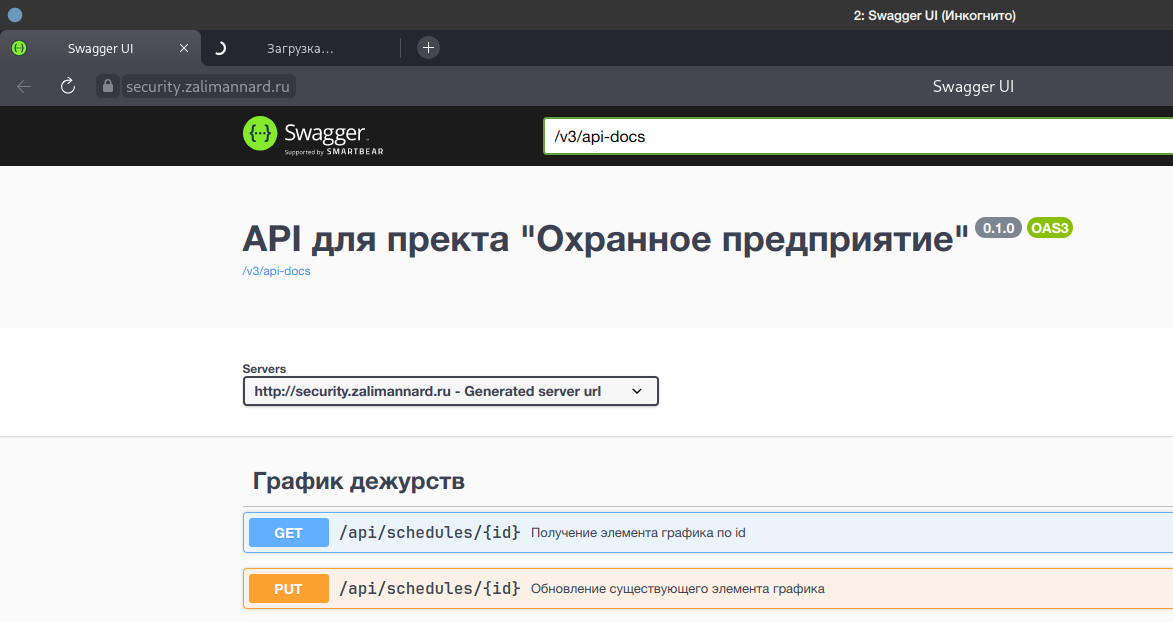
\includegraphics[width=0.8\linewidth]{Swagger.png}
        \caption{\centering Пример автоматической документации через Swagger}
        \label{fig:Swagger}
    \end{figure}

    У него есть уже упомянутые аннотации, как @Tag, которые позволяют составлять документацию ещё и в удобном для чтения формате. Присутствует возможность отправлять запросы прямо из этой панели.

    Главное преимущество автодокументирования -- то, что такая документация всегда актуальна. Она подстраивается под изменения кода и не может быть такого, что она устарела.

    \subsubsection{Тестирование}\label{Реализация. Сервер. Тестирование}

    Основной вид тестирования, которым нужно покрывать разрабатываемую систему -- интеграционное тестирование. Это вид тестирования, который позволяет удостовериться, что на конкретный запрос при конкретном состоянии системы возвращается заранее известный ответ. Таким образом, если все интеграционные тесты выполняются и они правильно написаны, то можно быть уверенным, что сервер работает правильно.

    Разработка тестов -- это отдельная большая часть работы над системой. Тестировать нужно не только уже разработанную систему на наличие ошибок. Тесты нужно создавать и проводить на протяжении всей разработки, причём, что важно -- до написания кода. Этот подход называется TDD (Разработка через тестирование) и является хорошей практикой в программировании, потому что тесты пишутся по техническому заданию и этапу проектирования, а не тогда, когда вся программа уже написана, потому что тесты будут подстраиваются под неё. Эффективность тестирования при TDD выше~\cite{cleancode}.

    Для данной системы тесты были разработаны в соответствии с TDD в отдельном Java-проекте. Можно сказать, что каждый из методов -- это эмуляция запроса клиента. Поэтому для них требуется наличие только DTO для запроса и ответа и путей к конечным точкам приложения. Так можно будет покрыть автоматическими тестами API всё приложение.

    Пример автоматического теста приведён на Листинге~\ref{test}. Здесь пользователь ADMIN, который создаётся по умолчанию при запуске создаёт пользователей с разными ролями. Все они должны создаться, тест позитивный. После завершения теста созданные данные удаляются -- это важный элемент в написании автотестов, ведь это сохраняет в чистоте тестовую среду и делает тесты более предсказуемыми и отслеживаемыми.

    \begin{lstlisting}[label=test,caption=Пример автотеста для разработанной системы]
    @ParameterizedTest
    @Severity(SeverityLevel.CRITICAL)
    @DisplayName("Invalid procedure name")
    @NullSource
    @ValueSource(strings = {"", " ", "   ", })
    void testPutProcedure_invalidName_BadRequest(String name) {
        ProcedureRequest existedProcedureRequest = ProcedureFactory.createProcedureRequest();
        ProcedureResponse existedProcedureResponse = procedureSteps.post(existedProcedureRequest, adminAuth);
        ProcedureRequest procedureToCreate = ProcedureFactory.createProcedureRequest().toBuilder()
            .name(name)
            .build();
        ErrorResponse actual = procedureSteps.put(
            existedProcedureResponse.getId(),
            procedureToCreate,
            adminAuth,
            specifications.responseSpecificationV1(400),
            ErrorResponse.class
        );
        assertThat(actual).isNotNull();
    }
    \end{lstlisting}

    Часто бывает необходимо не просто знать, что тест есть, а иметь возможность быстро понять что именно привело к непройденному тесту~\cite{springguide}. В таких случаях очень помогает специально средство для визуализации тестирования. В Gradle есть такой по умолчанию, но он не наглядный. Лучшая замена ему -- Allure. Он представляет результаты тестов в виде удобного отчёта. Пример отчёта Allure для разрабатываемой системы приведён на Рисунке~\ref{fig:Allure}.

    \begin{figure}[h]
        \centering
        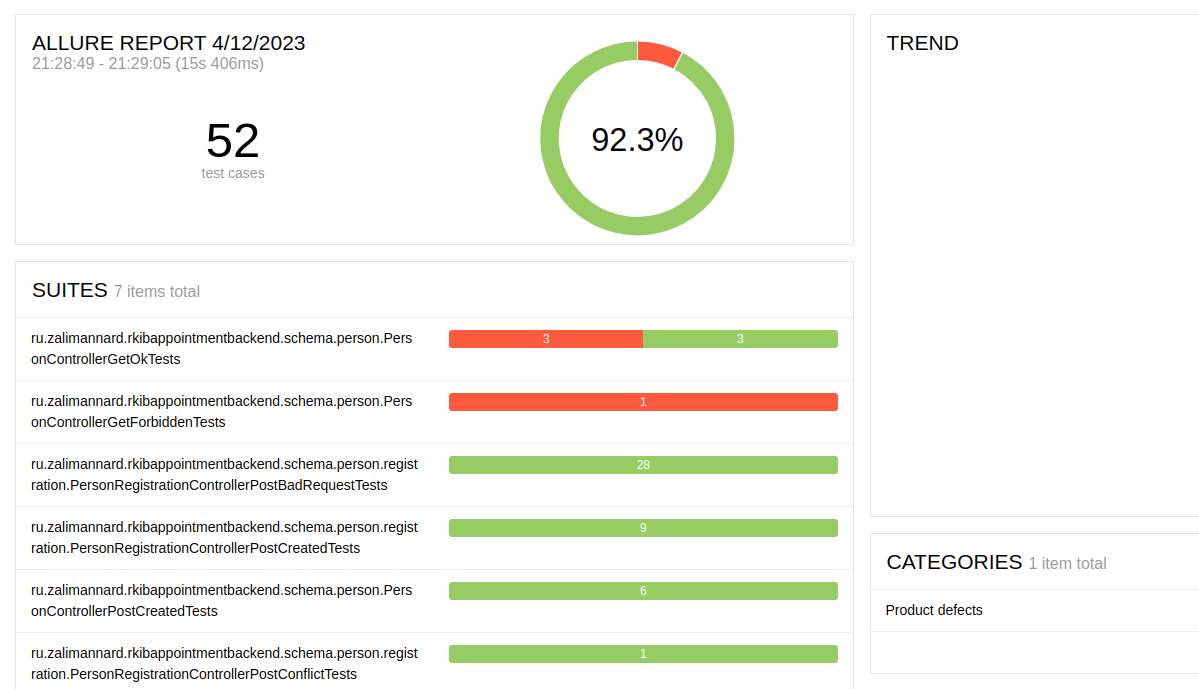
\includegraphics[width=0.8\linewidth]{Allure.png}
        \caption{\centering Пример визуализации результатов тестирования}
        \label{fig:Allure}
    \end{figure}

    Тесты бывают позитивные, которые проверяют нормальный ход работы системы, и негативные, которые проверяют правильность ошибки, появляющийся при том или ином действии. Большую часть всегда занимают негативные, потому что возможных сценариев ошибки значительно больше, чем сценариев нормальной работы~\cite{baeldungbook}. Это также отражено на Рисунке~\ref{fig:Allure}.

    \newpage

    \subsection{Клиентская часть}\label{Реализация. Клиентская часть}

    Последняя разрабатываемая часть -- клиентская. Предстоит реализовать пользовательский интерфейс и взаимодействие пользователя с серверное частью через него.

    \subsubsection{Структура проекта}\label{Реализация. Клиентская часть. Структура проекта}

    Рассмотрим структуру проекта. Она представлена на Листинге~\ref{frontendprojectstructure}, далее элементы разбираются подробнее~\cite{vuejs}.

    \begin{lstlisting}[label=frontendprojectstructure,caption=Структура клиентского приложения]
    views/
        admin/
        doctor/
        registrar/
    components/
        alert/
        button/
        dialog/
        select/
        table/
        textfield/
    plugins/
    router/
    types/
    backspaceHandlers.ts
    main.ts
    masks.ts
    rules.ts
    utils.ts
    \end{lstlisting}

    Папка views содержит страницы приложения в формате <<.vue>>, то есть содержат код на HTML, TypeScript и CSS одновременно.

    Components содержит элементы приложения, которые можно выделить и переиспользовать. Так, для кнопки можно выделить отдельный компонент, чтобы на всё приложение только один раз задать степень закругления и общий стиль кнопки. Либо, например, элемент уведомлений должен быть один на всё приложение. Для него тоже стоит сделать отдельный компонент. А вынос в свои компоненты текстового поля поможет не писать вручную каждый раз правила взаимодействия с правилами, которые рассмотрим ниже.

    Далее для взаимодействия клиента и сервера на стороне клиента также необходимо объявить объекты, которые будут использоваться для отправки запросов и приёма ответов. Пример -- на Листинге~\ref{customtype}~\cite{vuejs}.

    \begin{lstlisting}[label=customtype,caption=Пример объявленных типов для обмена сообщениями с сервером]
    export interface AppointmentStatusRequest {
        name: string;
        type: string;
    }
    export interface AppointmentStatusResponse {
        id: string;
        name: string;
        type: string;
    }
    \end{lstlisting}

    Рассмотрим одну из главных папок -- router~\cite{vuejs}. Она содержит в себе информацию о том, какой конечной точке какой компонент соответствует. Конкретно -- те, которые хранятся в папке views.

    Из важных для разработки элементов можно выделить ещё 3 файла -- <<backspaseHandlers>>, <<masks>> и <<rules>>. Они отвечают за то, чтобы в текстовые поля были заполнены правильными данными. Яркий пример -- номер телефона. Формат номера <<+7(123)456-78-90>> читается удобнее, чем <<+71234567890>> При этом важно не просто давать пользователю удобно вводить номер, но и удалять. Чтобы ему не приходилось удалять автоматически сгенерированные символы <<(>>, <<.>> и подобные. Наконец, нужно проверять написанный/сконвертированный номер на корректность, чем занимаются методы в файле rules. Пример для номера телефона представлен на Листинге~\ref{phonerule}. Указание пустой строки, либо <<+7>> означает отсутствие номера. Любая другая строка кроме имеющих формат <<+7(XXX)XXX-XX-XX>>, где X -- цифра, не является корректным номером телефона.

    \newpage

    \begin{lstlisting}[label=phonerule,caption=Пример проверки корректности телефона]
    export const phoneRule: Rule[] = [
        (value: string) => {
            if (!value) return true;
            if (value === "+7(") return true;
            const pattern = /^\+7\((\d{3})\)(\d{3})-(\d{2})-(\d{2})$/;
            if (!pattern.test(value)) return "Incomplete number";
            return true;
        }
    ];
    \end{lstlisting}

    \subsubsection{Архитектура приложения}\label{Реализация. Клиентская часть. Архитектура слоёв}

    В пункте~\ref{Реализация. Клиентская часть. Структура проекта} рассмотрены основные элементы системы и где они хранятся. Теперь рассмотрим архитектуру системы. Основная схема представлена на Рисунке~\ref{fig:Схема работы клиента}.

    \begin{figure}[h]
        \centering
        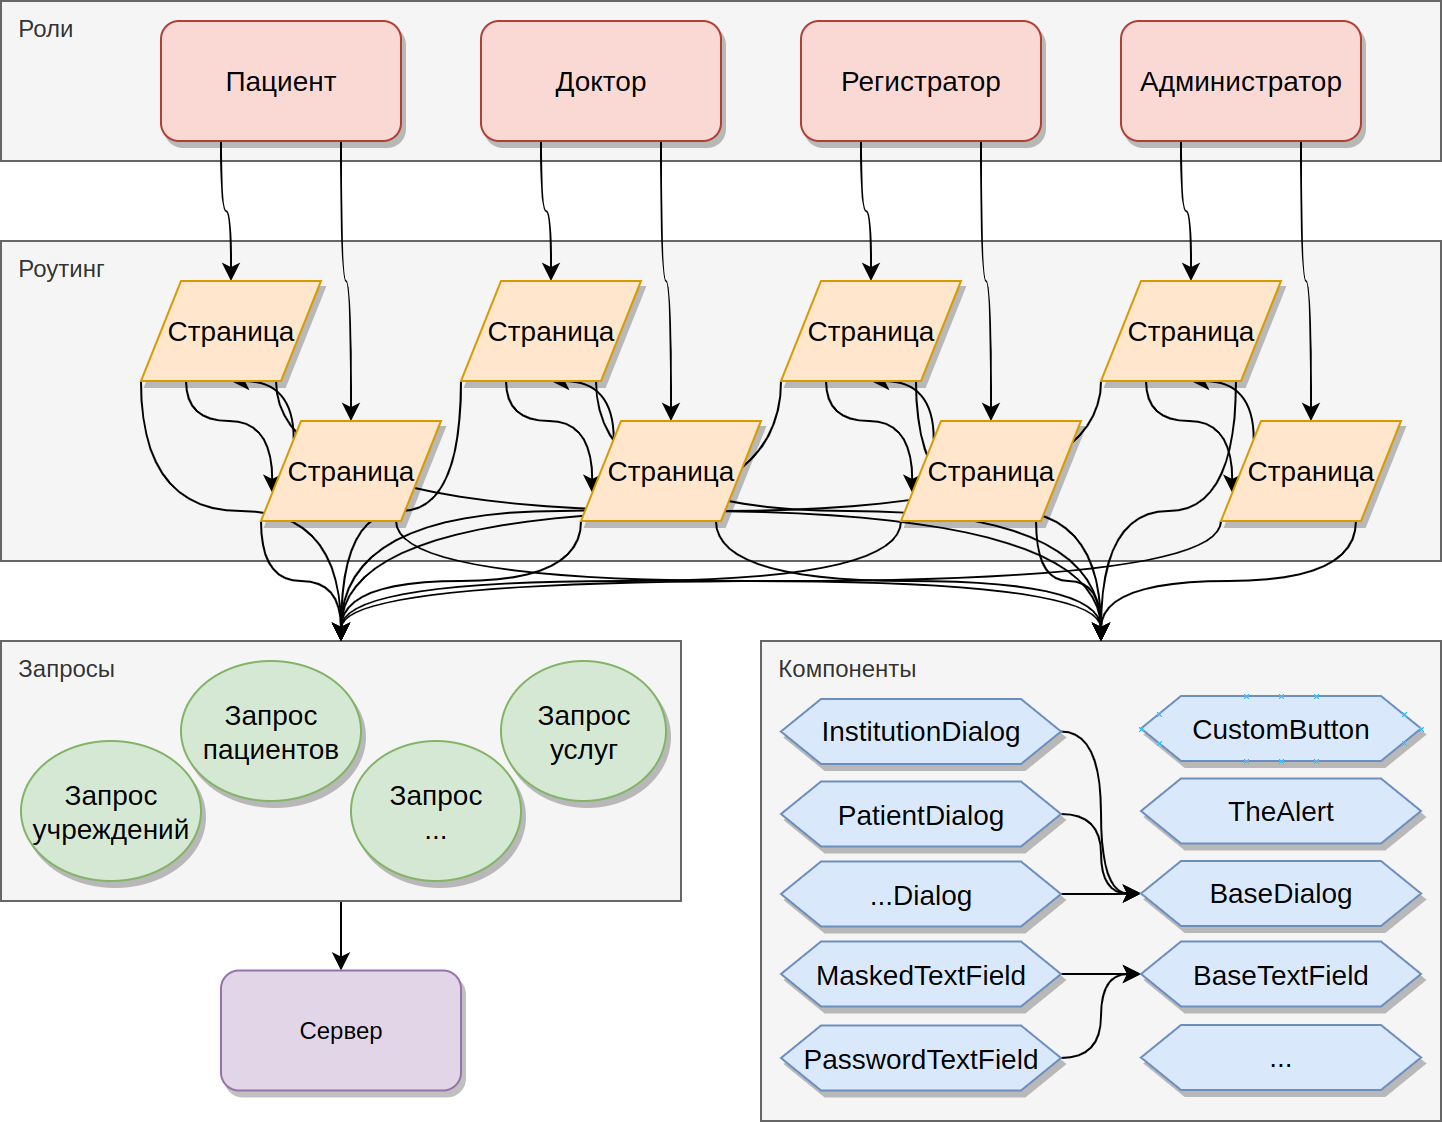
\includegraphics[width=0.9\linewidth]{Схема работы клиента.png}
        \caption{\centering Схема работы клиента}
        \label{fig:Схема работы клиента}
    \end{figure}
    
    \newpage

    Изображено взаимодействие элементов системы -- пользователь под конкретной ролью перемещается по страницам, которые, в свою очередь, через API-запросы передают и получают информацию с сервера. К тому же эти страницы состоят из переиспользуемых компонентов, некоторые из которых расширяют функционал других, более общих.

    Элемент <<Сервер>> соответствует схеме с Рисунка~\ref{fig:Схема работы сервера}, если из него убрать <<Клиент>>, поскольку клиент -- это основная часть этого рисунка. Эти схемы дополняют друг друга.

    \subsubsection{Пользовательский интерфейс}\label{Реализация. Клиентская часть. Пользовательский интерфейс}
    
    В соответствии с определёнными ранее требованиями к интерфейсу, реализован интерфейс. По порядку разберём его части. 
    
    Первое, конечно же, вход в систему. Представлен на Рисунке~\ref{fig:uilogin}. Поскольку у сотрудника может быть несколько ролей, то он может выбрать -- под какой именно ролью он хочет сейчас работать.
    
    \begin{figure}[h]
        \centering
        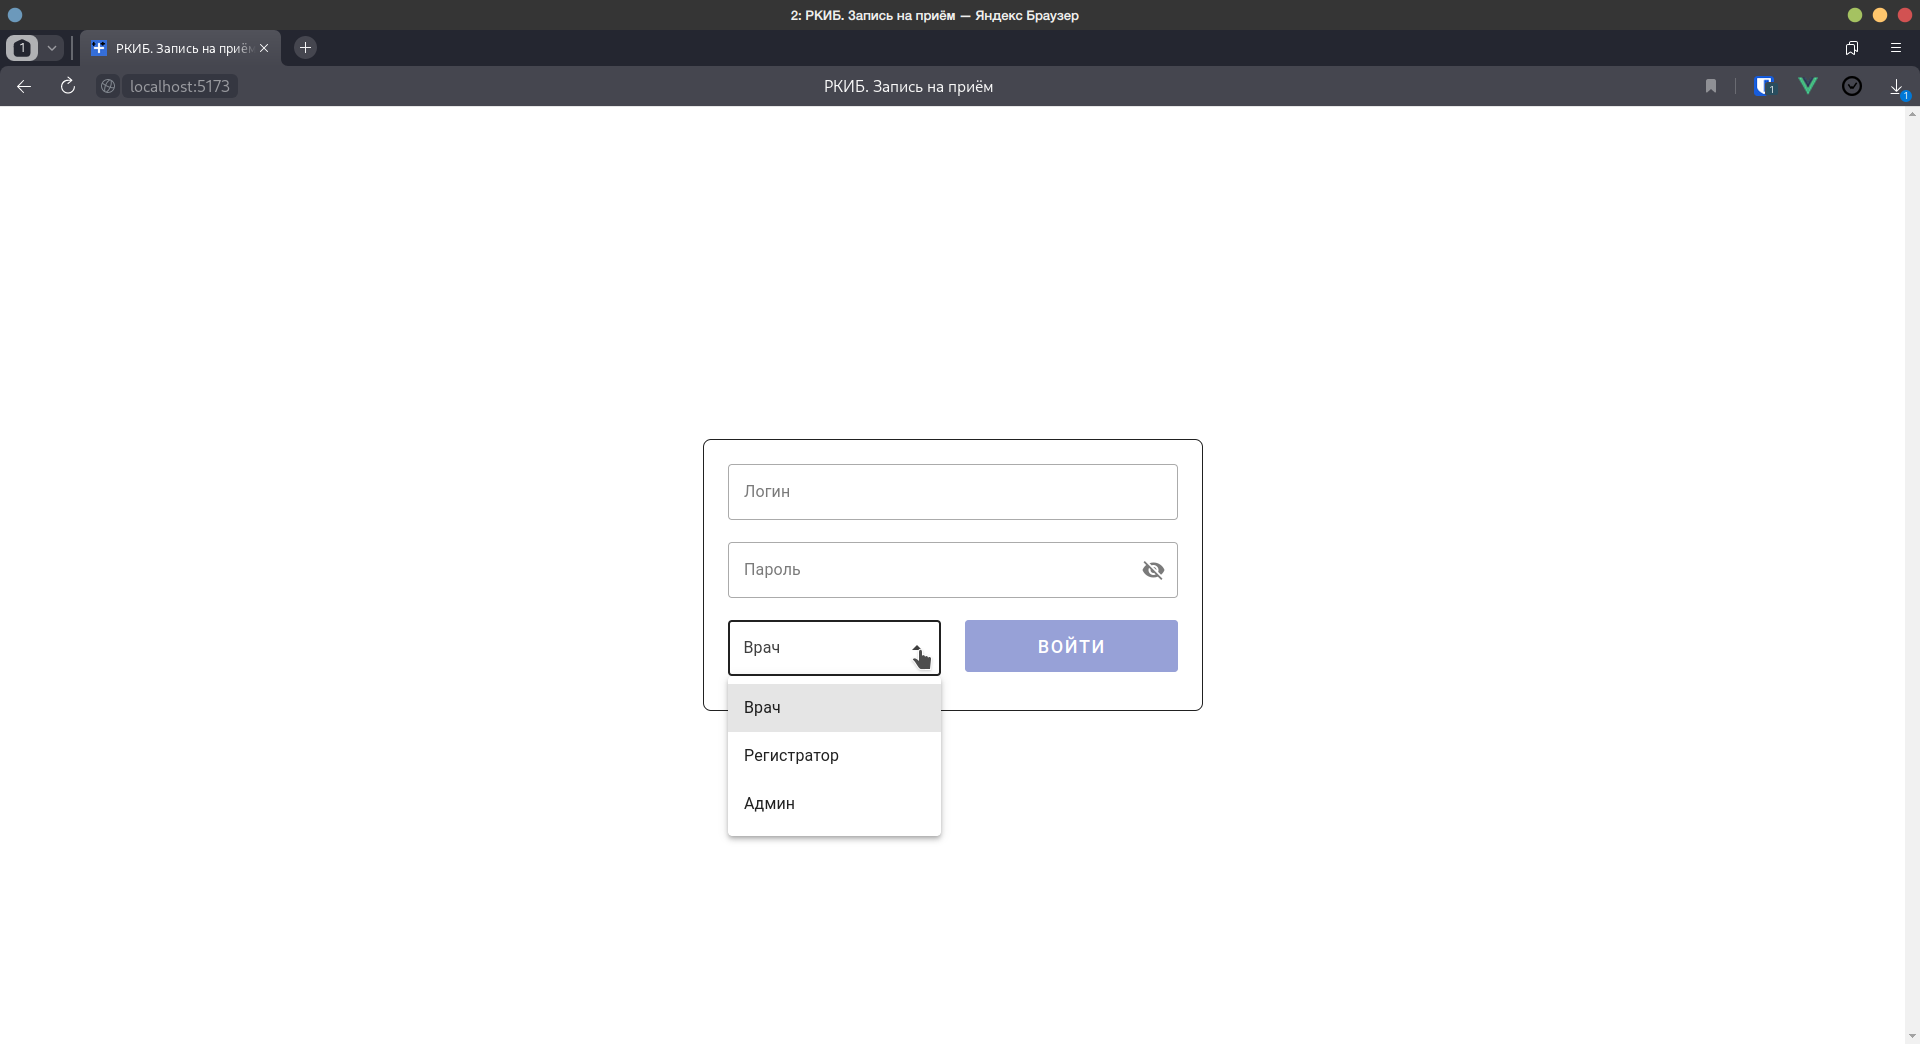
\includegraphics[width=0.8\linewidth]{UI. Вход как сотрудник.png}        
        \caption{\centering Вход в систему как сотрудник}        
        \label{fig:uilogin}        
    \end{figure}
    
    \newpage
    
    Если во время работы с системой произошла ошибка, то появится уведомление об этом, как на Рисунке~\ref{fig:uierror}
    
    \begin{figure}[h]
        \centering
        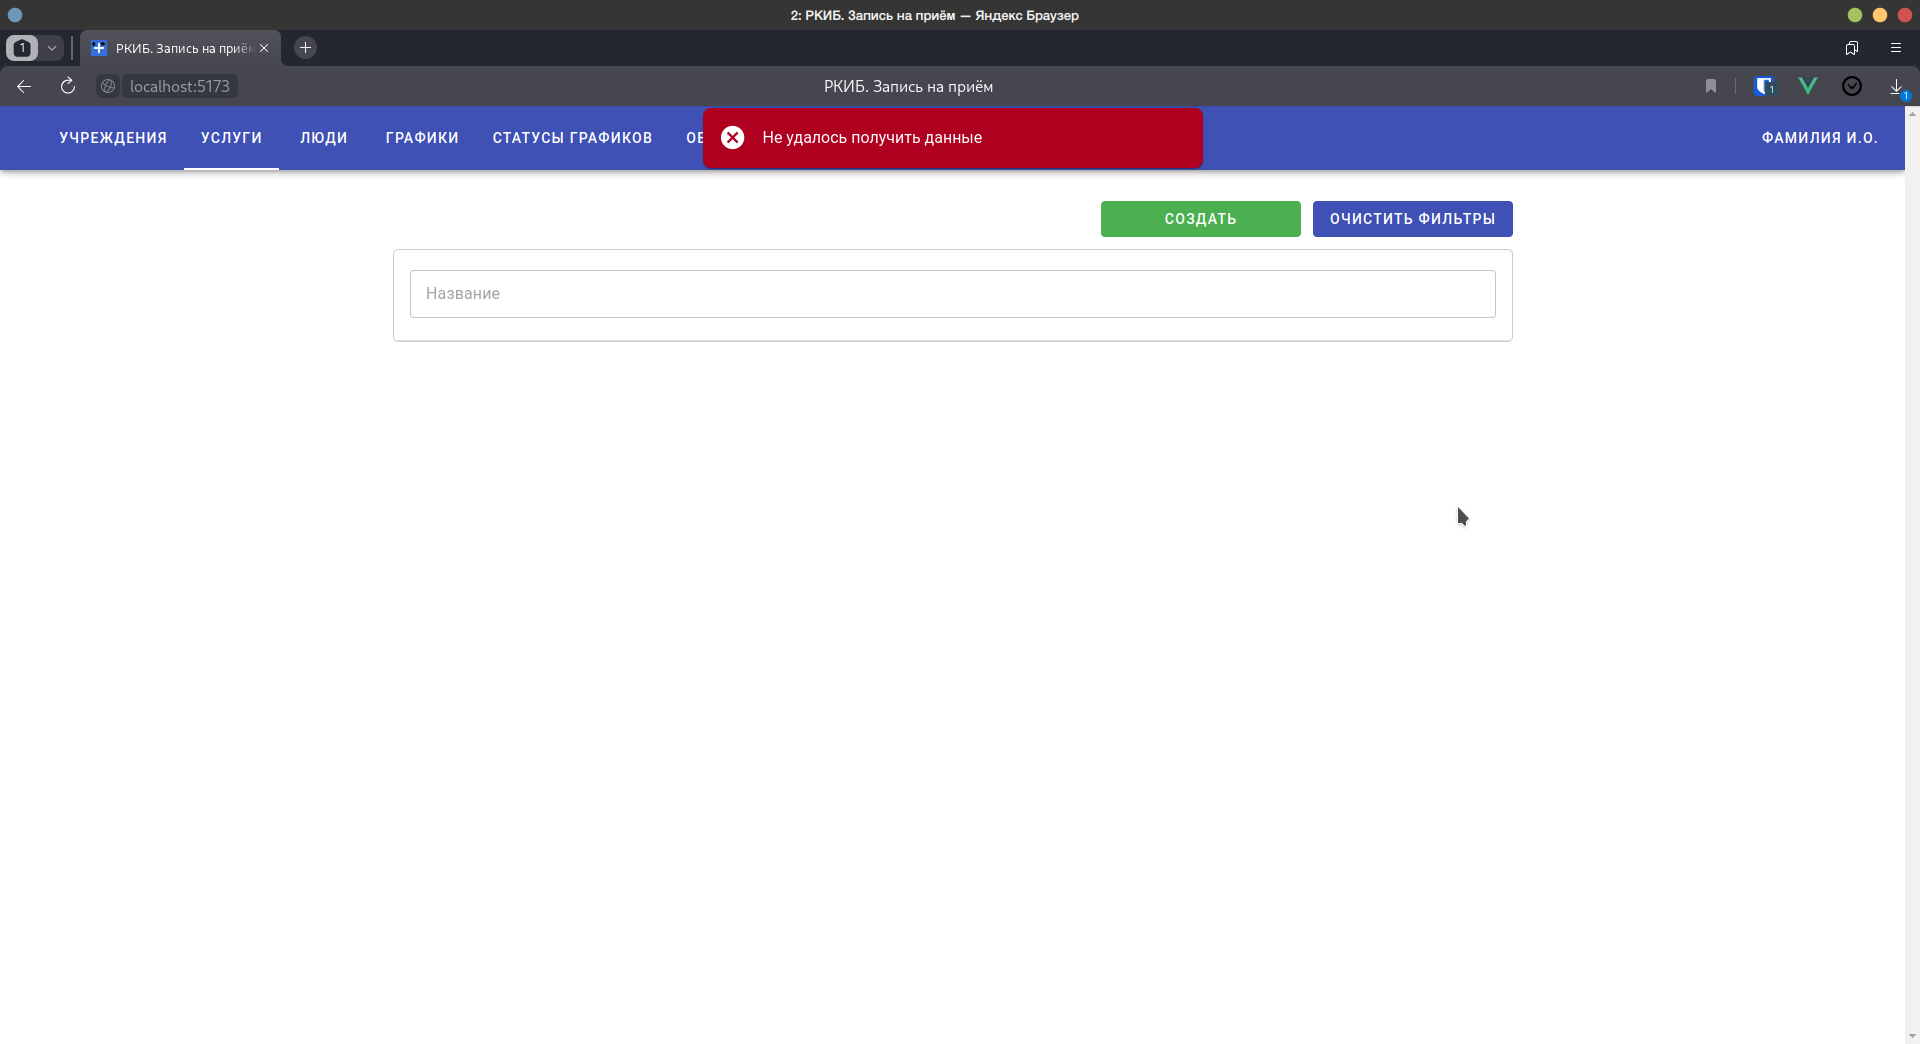
\includegraphics[width=0.8\linewidth]{UI. Пример ошибки.png}        
        \caption{\centering Пример ошибки при работе с системой}        
        \label{fig:uierror}        
    \end{figure}
    
    Если же страница загружена нормально, то появится её содержимое. Пример для таблицы. После этого можно вводить различные данные в фильтры и список будет обновляться. Если фильтрация должна быть не простому полю, а по другому объекту, то появляется окно с выбором элемента с возможностью нажатия, что можно увидеть на Рисунке~\ref{fig:uiappointment}
    
    \begin{figure}[h]
        \centering
        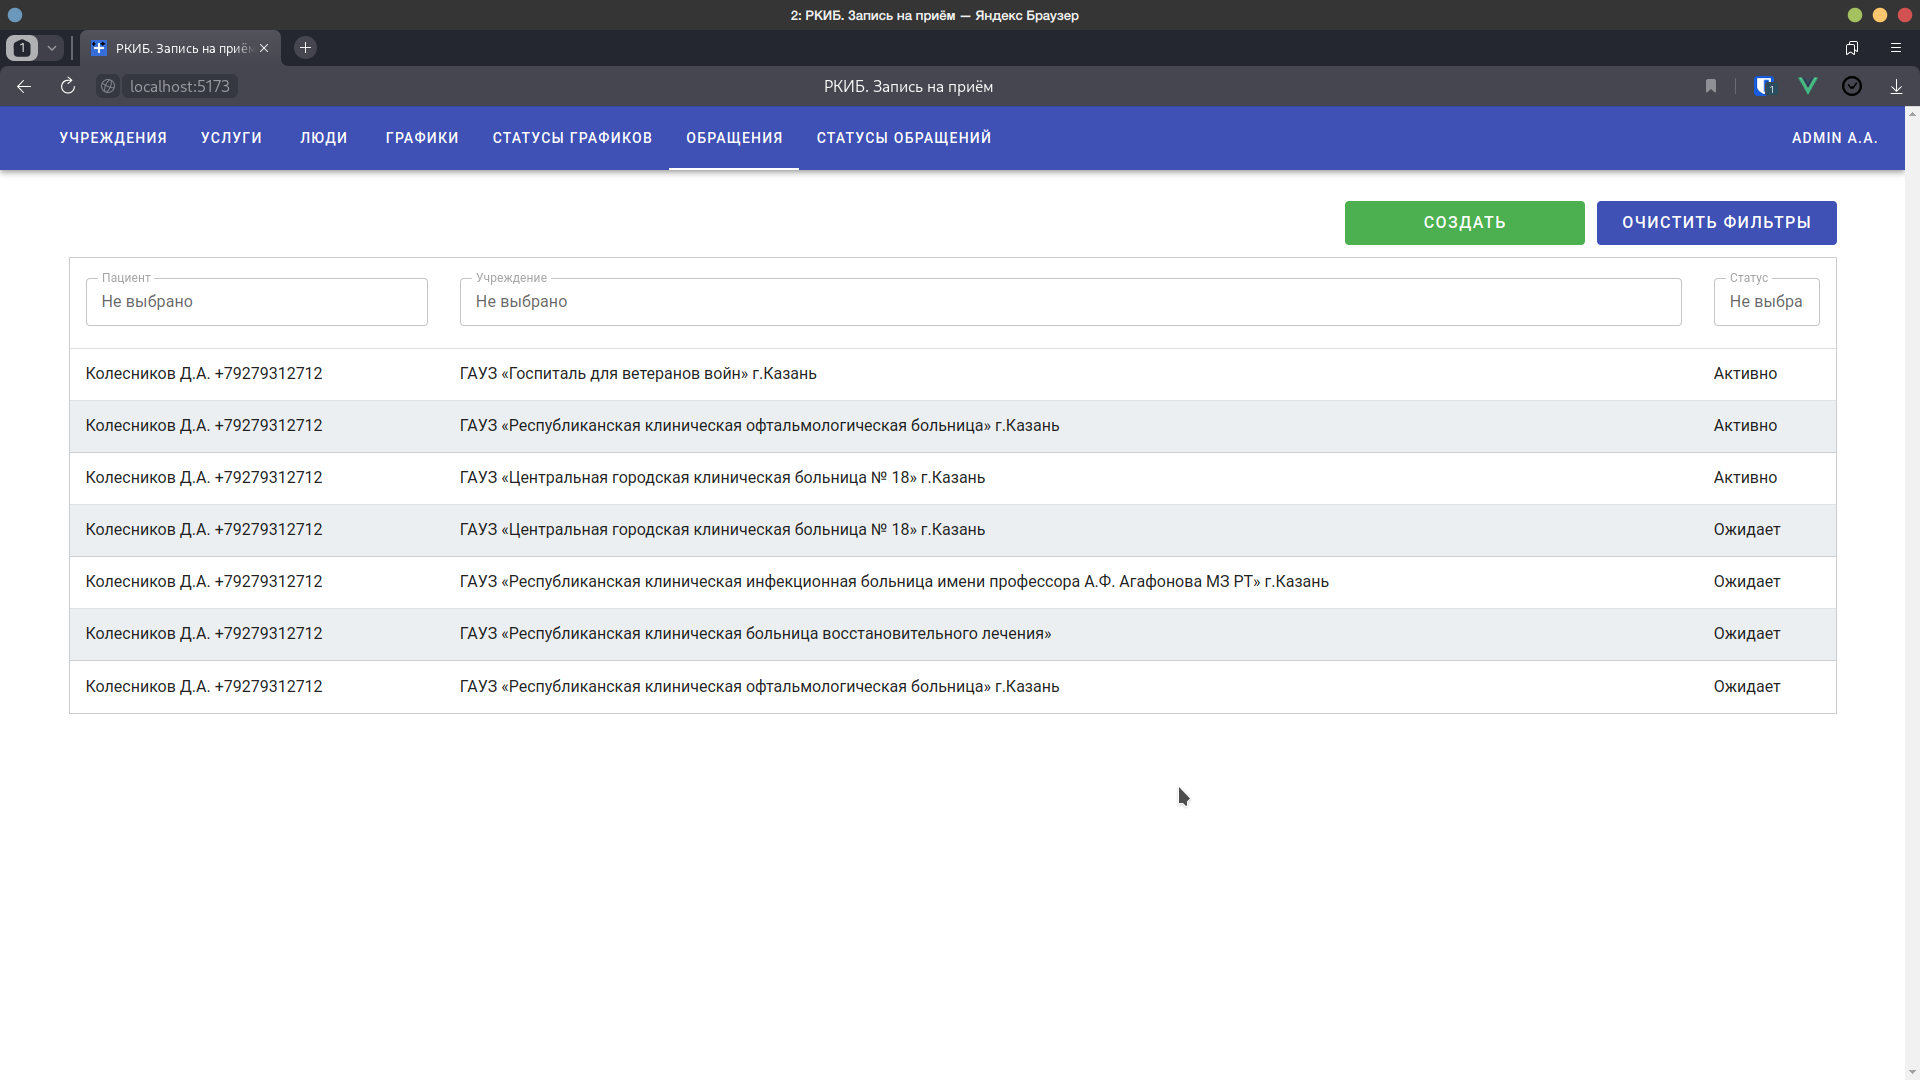
\includegraphics[width=0.8\linewidth]{UI. Обращения от ADMIN.png}        
        \caption{\centering Пример страницы с обращениями от Администратора}        
        \label{fig:uiappointment}        
    \end{figure}
    
    \newpage
    
    Присутствует возможность создавать новые элементы. В таком случае появляется такой как на Рисунке~\ref{fig:uiadd} или подобный диалог с нужными параметрами
    
    \begin{figure}[h]
        \centering
        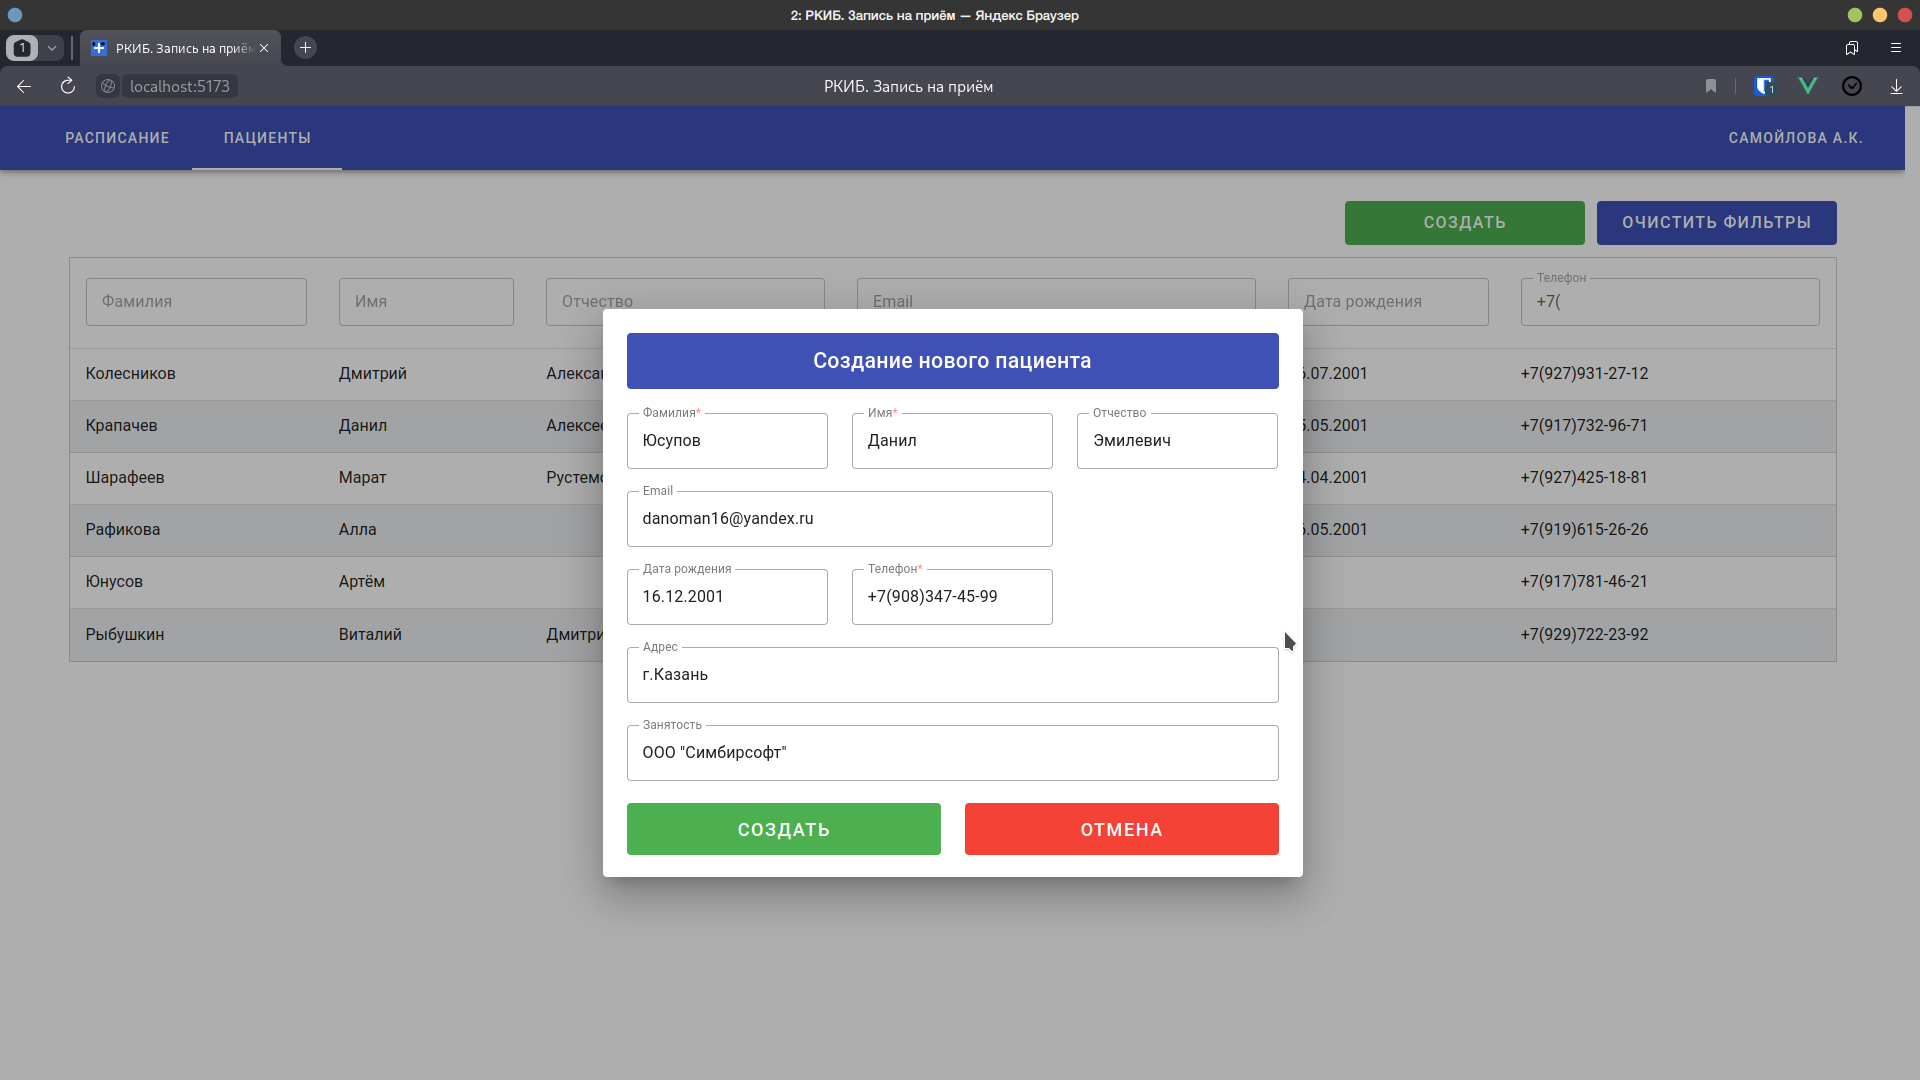
\includegraphics[width=0.8\linewidth]{UI. Создание человека.png}        
        \caption{\centering Интерфейс для создания человека регистратором}        
        \label{fig:uiadd}        
    \end{figure}
    
    Интерфейс создания своего расписания представлен на Рисунке~\ref{fig:createsched}. Можно выбрать временной интервал, промежуток между приёмами, дни и услугу.
    
    \begin{figure}[h]
        \centering
        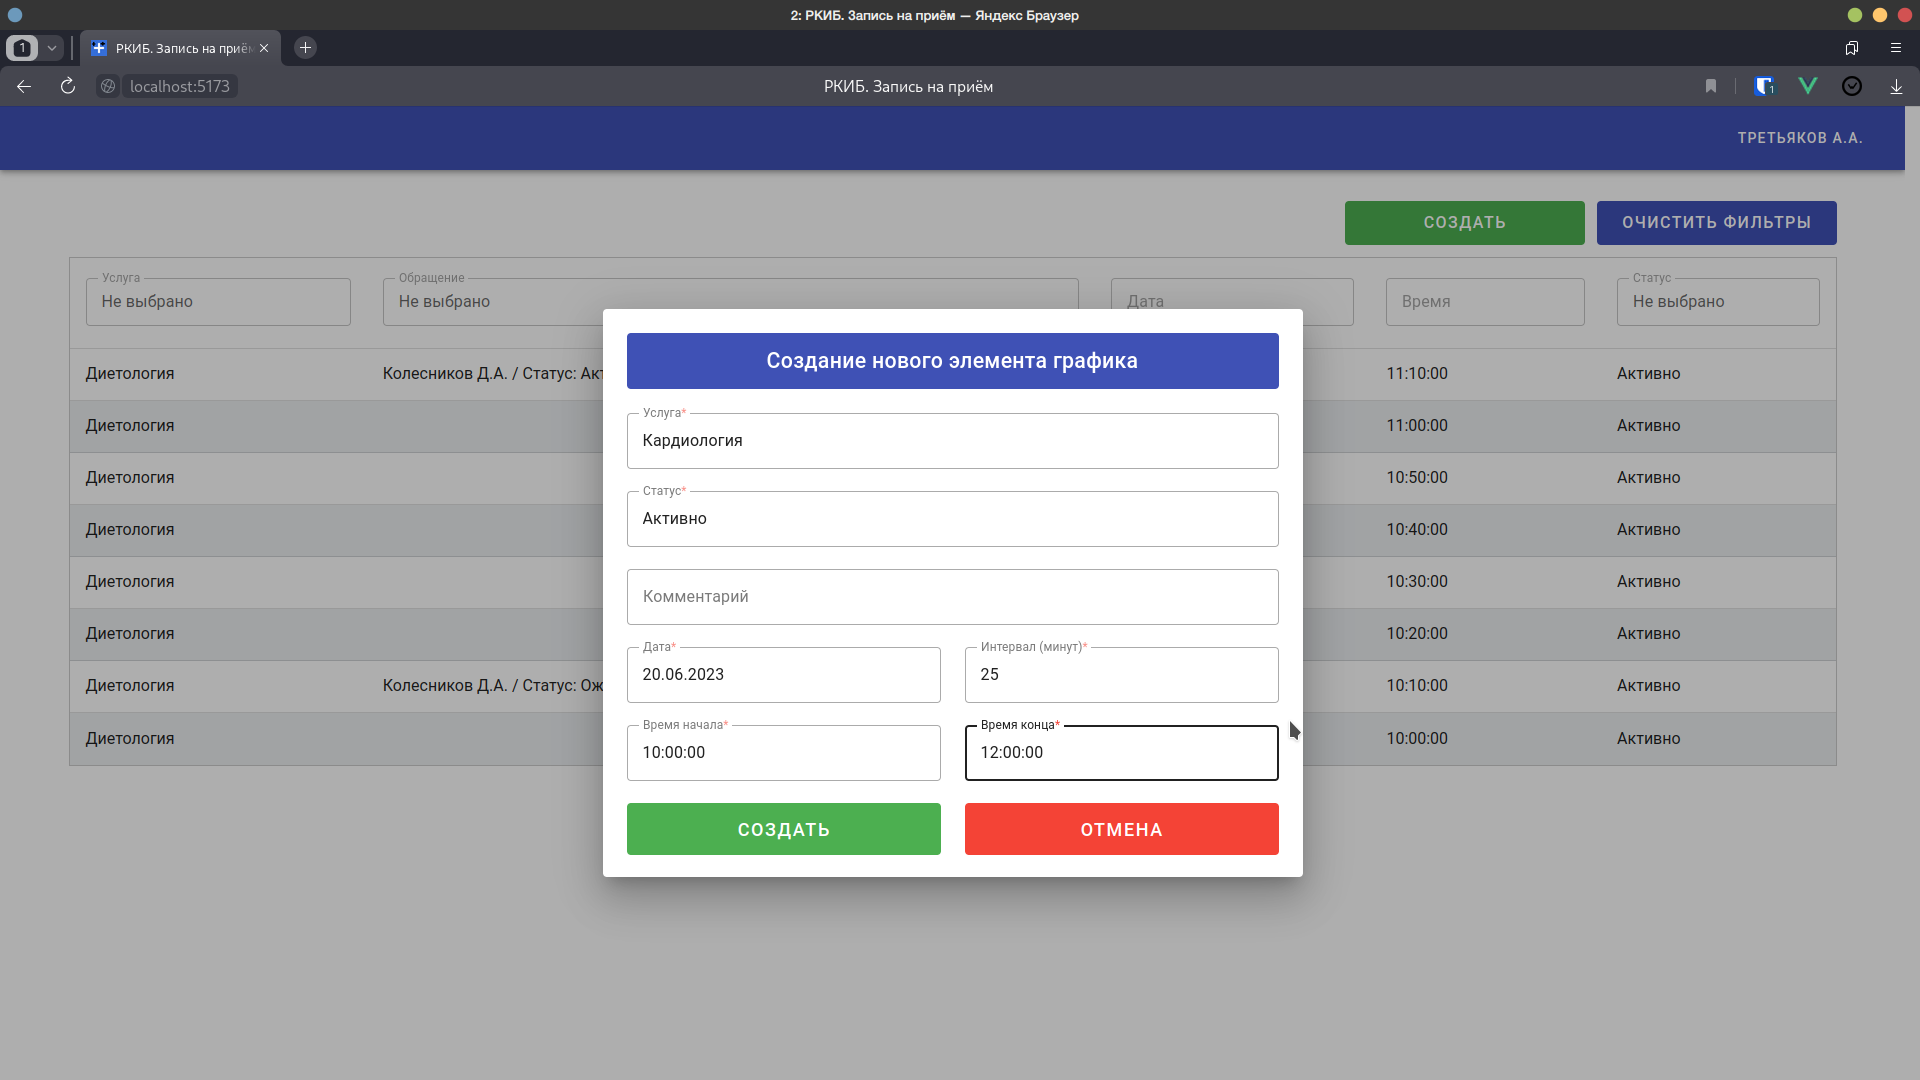
\includegraphics[width=0.8\linewidth]{UI. Пример создания расписания.png}        
        \caption{\centering Интерфейс для создания расписания}        
        \label{fig:createsched}        
    \end{figure}
    
    \newpage
    
    На Рисунке~\ref{fig:dosched} показано как выглядит интерфейс уже показа созданных элементов расписания. Видно какое время занято, какое свободно. Можно выбрать и отправить заявку регистратору.
    
    \begin{figure}[h]
        \centering
        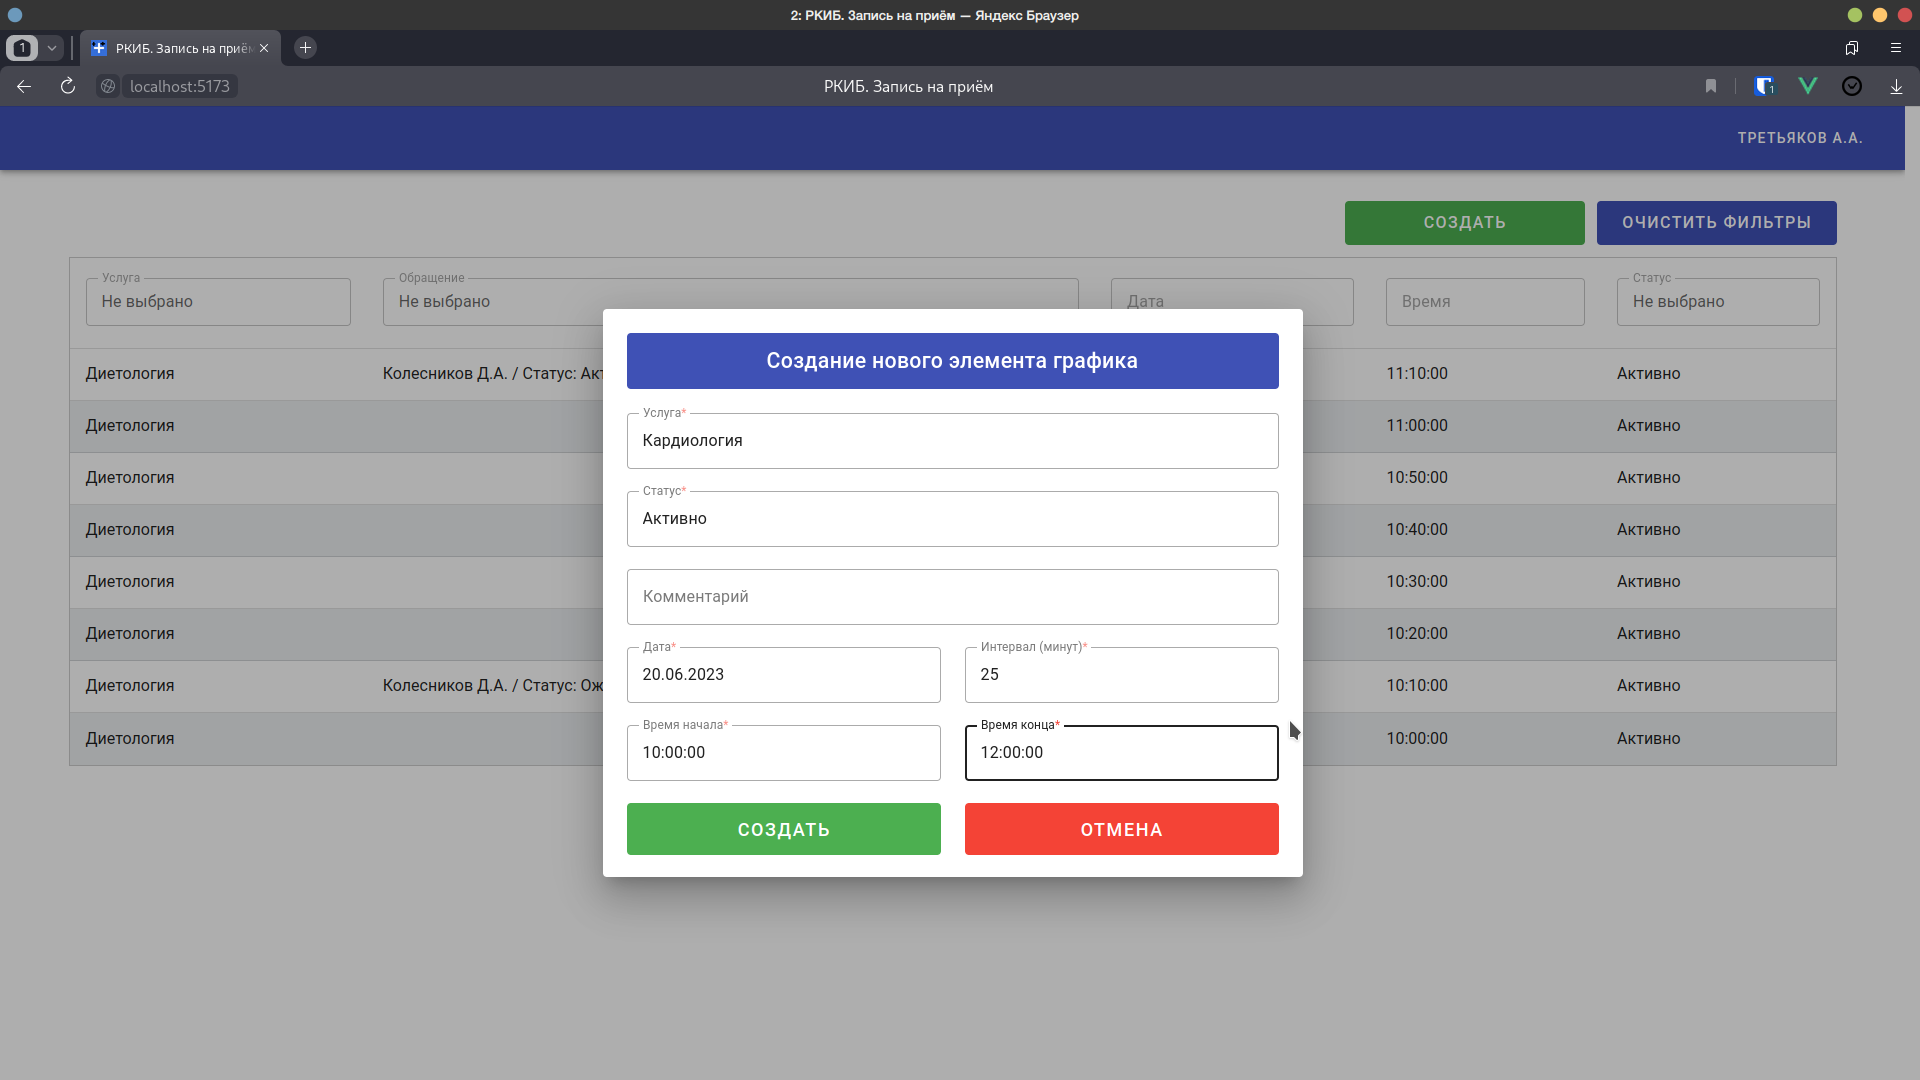
\includegraphics[width=0.8\linewidth]{UI. Пример создания расписания.png}        
        \caption{\centering Интерфейс для создания расписания}        
        \label{fig:dosched}
    \end{figure}

    \subsubsection{Тестирование}\label{Реализация. Клиентская часть. Тестирование}
    
    Тестирование пользовательского интерфейса будет производиться через Selenide -- удобную обёртку для Selenium. С его помощью можно писать пошагово действия в тестах и обозначать ожидаемое поведение. Пример -- на Листинге~\ref{selenide}. Когда возможно - лучше обращаться к элементам через id, class, text и прочие параметры. В приведённом листинге это строки 4-5. Далее показывается менее желательное, но гарантированное нахождение элементов -- через xpath. Это полный путь до объекта, с которым нужно взаимодействовать.
    
    \newpage
    
    \begin{lstlisting}[label=selenide,caption=Пример теста на Selenide]
    @Test
    void loginTest() {
      open(startUrl);
      $(By.id("email")).setValue("admin@admin.ru");
      $(By.id("password")).setValue("admin");
      $(By.xpath("//*[@id=\"app\"]/div/div/main/div/div/div/form/div[3]/div[1]/div")).click();
      $(By.xpath("/html/body/div[2]/div/div/div/div[3]")).click();
      $(By.xpath("//*[@id=\"app\"]/div/div/main/div/div/div/form/div[3]/div[2]/button")).click();
      $(By.xpath("//*[@id=\"app\"]/div/div/main/div/div/header/div/div[1]/div/div/a[5]")).click();
      $(By.xpath("//*[@id=\"app\"]/div/div/main/div/div/main/div/div/div[1]/div/button[1]")).shouldHave(text("СЗДТ"));
    }
    \end{lstlisting}
    
    Проваленные написанные тесты визуализируются с помощью Allure с плагином для Selenide~\cite{allure}. Если тест провален, то автоматически делается скриншот, который потом можно посмотреть, как на Рисунке~\ref{fig:allure}. Скриншот и код страницы сохраняются, если тест провален. Для всех тестов сохраняется последовательность действий.
    
    \begin{figure}[h]
        \centering
        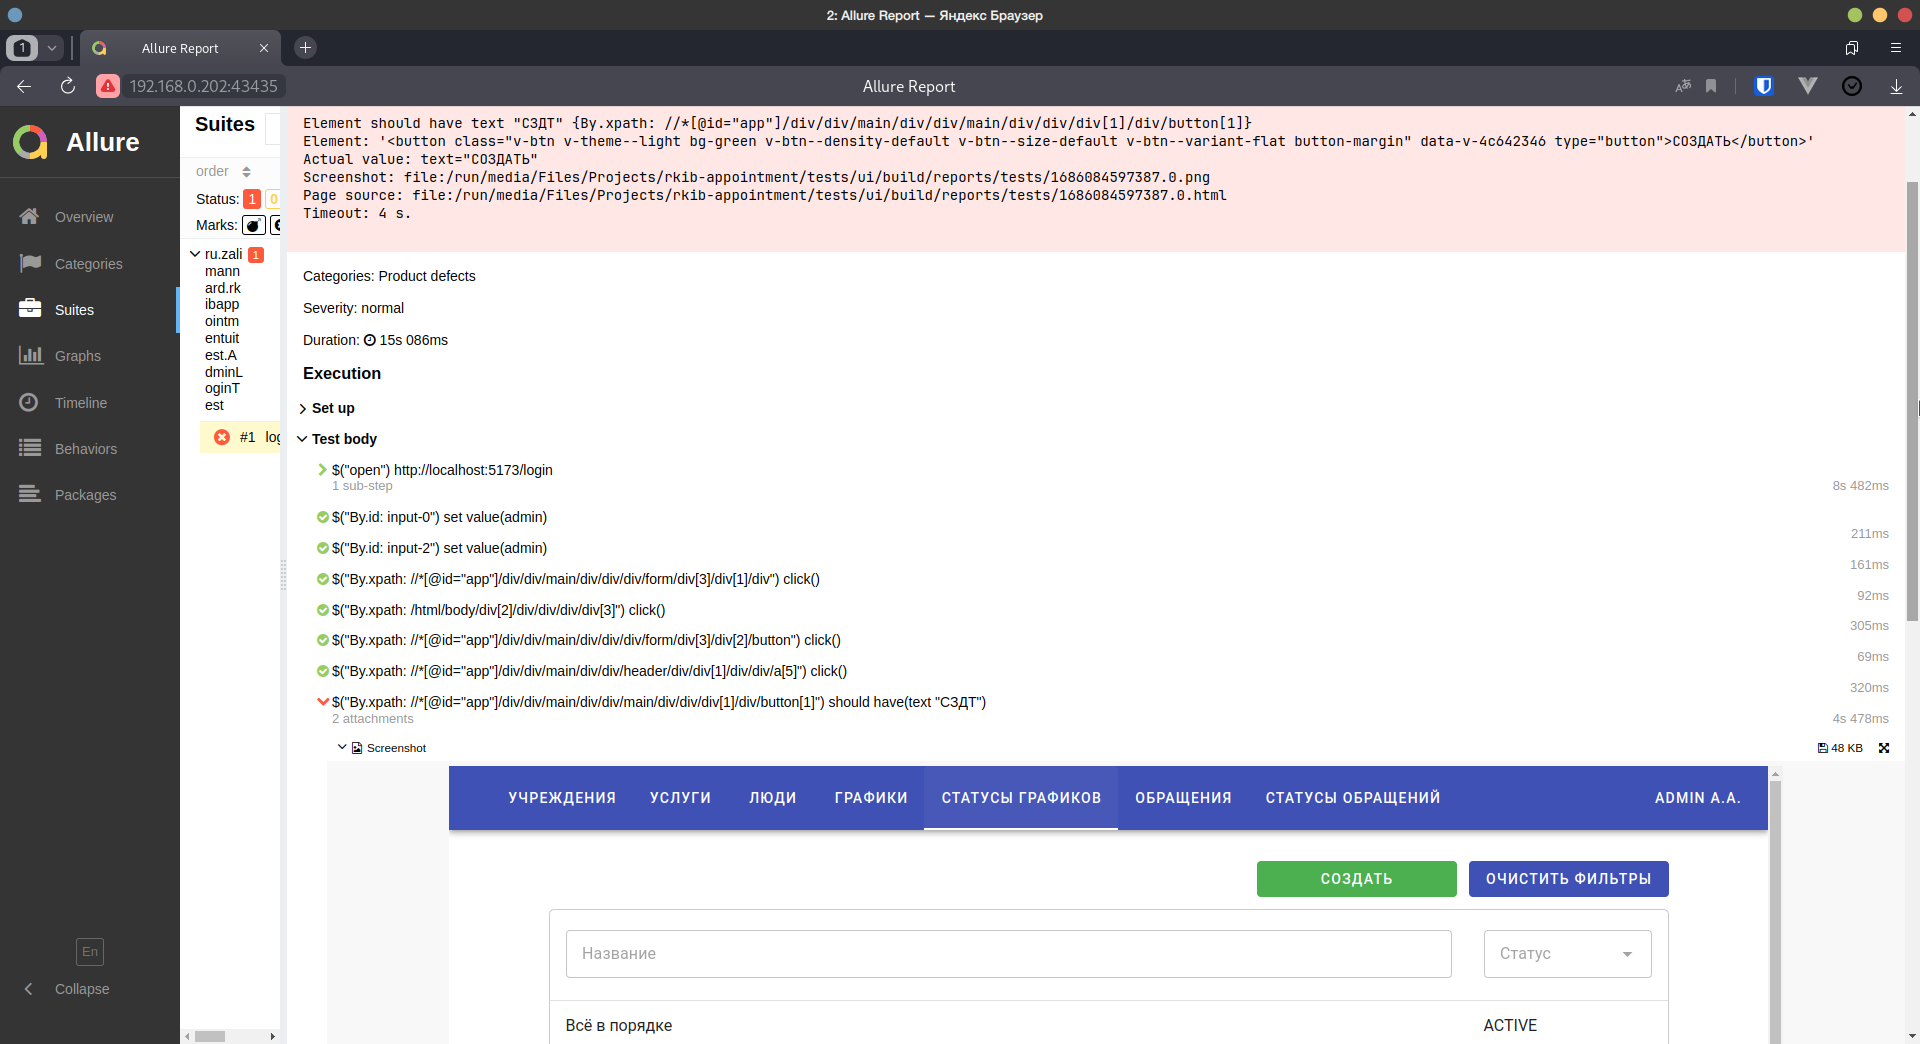
\includegraphics[width=0.8\linewidth]{UI. Отчёт Allure.png}        
        \caption{\centering Пример отчёта Allure о проваленном UI-тесте}        
        \label{fig:allure}
    \end{figure}
    
    \newpage

    \subsection{Развёртывание системы}\label{Реализация. Сборка и развертывание}
    
    Для каждой из частей приложения есть возможность запустить его через Docker~\cite{dockerdoc}. Образы загружены на DockerHub, то есть их можно удобно загрузить и сразу запустить.
    
    Для разворачивания приложения необходим docker-compose. Нужно создать основной файл, где будут указаны контейнеры и их параметры -- docker-compose.yml. Примерное содержимое этого файла представлено в Приложении~2. Далее нужно вставить свои данные, если они нужны, в параметры в environment.
    
    Всё, что остаётся делать дальше -- запустить приложение командой <<docker-compose up -d>> в консоли и система будет готова к работе.

    \newpage

    \section*{Заключение}
    \addcontentsline{toc}{section}{Заключение}
    
    Результатом работы является разработанное клиент-серверное приложение для записи на приём в медицинское учреждение.
    
    Для реализации изучены предметная область больницы на примере РКИБ, освоены теоретические и практические навыки по написанию частей клиент-серверного приложения. 
    
    Серверная часть разработана на Java с помощью фреймворка Spring. В качестве системы управления базами данных используется Oracle, взаимодействие с ней осуществляется через JPA. С помощью подхода TDD и инструмента RestAssured написаны интеграционные тесты и код, реализующий API для них.
    
    Клиентская часть разработана на языке TypeScript с использованием фреймворка Vue и фреймворка компонентов Vuetify. Протестировано с помощью Selenide и ошибки визуализируются с помощью Allure и плагина Selenide для него.
    
    Разворачиваются части приложения с помощью Docker. Написана инструкция по разворачиванию приложения на любом компьютере с Docker и docker-compose.
    
    Исходный код всех частей приложения, тестов, а также этого текста находится на GitHub: https://github.com/zalimannard/rkib-appointment

    \newpage

    \section*{Список использованных источников}
    \addcontentsline{toc}{section}{Список использованных источников}

    \begin{enumerate}[leftmargin=*, itemindent=\labelwidth]
        
        \bibitem{allure} Allure Framework [Электронный ресурс] -- URL: \url{https://docs.qameta.io/allure-report/} (Дата обращения: 22.05.2023)
        
        \bibitem{dbdiag} Database diagrams [Электронный ресурс] -- URL: \url{https://drawsql.app/diagrams} (Дата обращения: 17.11.2022)
        
        \bibitem{oracle} Database Express Edition Getting Started Guide [Электронный ресурс] -- URL: \url{https://docs.oracle.com/cd/E17781_01/admin.112/e18585/toc.htm#XEGSG101} (Дата обращения: 16.10.2022)
        
        \bibitem{dockerdoc} Docker Documentation [Электронный ресурс] -- URL: \url{https://docs.docker.com/} (Дата обращения: 05.03.2023)
        
        \bibitem{baeldungbook} Eugen. Build your API with Spring [Электронный ресурс] -- URL: \url{https://www.baeldung.com/rest-api-spring-guide} (Дата обращения: 01.12.2022)
        
        \bibitem{lombok} Project Lombok [Электронный ресурс] -- URL: \url{https://projectlombok.org/} (Дата обращения: 16.10.2022)
        
        \bibitem{restassured} REST Assured [Электронный ресурс] -- URL: \url{https://rest-assured.io/} (Дата обращения: 21.01.2023)
        
        \bibitem{selenide} Selenide: лаконичные и стабильные UI тесты на Java [Электронный ресурс] -- URL: \url{https://ru.selenide.org/} (Дата обращения: 03.04.2023)
        
        \bibitem{springguide} Spring | Guides [Электронный ресурс] -- URL: \url{https://spring.io/guides} (Дата обращения: 12.01.2023)
        
        \bibitem{vite} Vite | Next Generation Frontend Tooling [Электронный ресурс] -- URL: \url{https://ru.vuejs.org} (Дата обращения: 03.04.2023)
        
        \bibitem{vuejs} Vue.js -- Прогрессивный JavaScript-фреймворк [Электронный ресурс] -- URL: \url{https://ru.vuejs.org} (Дата обращения: 03.04.2023)
        
        \bibitem{vuetify} Vuetify -- A Vue Component Framework [Электронный ресурс] -- URL: \url{https://vuetifyjs.com/en/getting-started/installation/} (Дата обращения: 03.04.2023)
        
        \bibitem{tdd} What is TDD? What is Unit Testing? - Simple Programmer [Электронный ресурс] -- URL: \url{https://simpleprogrammer.com/tdd-unit-testing/} (Дата обращения: 13.02.2023)
        
        \bibitem{webapi} Грамотная клиент-серверная архитектура: как правильно проектировать и разрабатывать web API [Электронный ресурс] -- URL: \url{https://tproger.ru/articles/web-api/} (Дата обращения: 03.11.2022)
        
        \bibitem{apitypes} Исчерпывающее руководство по различным типам API [Электронный ресурс] -- URL: \url{https://habr.com/ru/companies/otus/articles/737610/} (Дата обращения: 28.10.2022)
        
        \bibitem{httpadderrors} Как работать с ошибками бизнес-логики через HTTP [Электронный ресурс] -- URL: \url{https://habr.com/ru/articles/545524/} (Дата обращения: 22.04.2023)
        
        \bibitem{cleanarch} Мартин Р. Чистая архитектура. Искусство разработки программного обеспечения. -- СПб.: Питер, 2022. -- 352 с.
        
        \bibitem{cleancode} Мартин Р. Чистый код: создание, анализ и рефакторинг. -- СПб.: Питер, 2022. -- 464 с.
        
        \bibitem{dbdesign} Осипов Д.Л. Технологии проектирования баз данных. -- М.: ДМК Пресс, 2019. -- 498 с.
        
        \bibitem{1cmedicine} Решения 1С для отрасли: Здравоохранение и медицина [Электронный ресурс] -- URL: \url{https://solutions.1c.ru/med} (Дата обращения: 03.10.2022)
        
        \bibitem{httpstatus} Список кодов состояния HTTP [Электронный ресурс] -- URL: \url{https://ru.wikipedia.org/wiki/Список_кодов_состояния_HTTP} (Дата обращения: 13.01.2023)
        
        \bibitem{backstack} Топ 10 Технологий для Бэкенд Разработки [Электронный ресурс] -- URL: \url{https://blog.back4app.com/ru/топ-10-технологий-для-бэкенд-разработки/} (Дата обращения: 24.11.2022)
        
        \bibitem{natsproektzdravoohranenie} Федеральный проект <<Создание единого цифрового контура в здравоохранении на основе единой государственной информационной системы в сфере здравоохранения (ЕГИСЗ)>> -- 2019 -- 9 августа [Электронный ресурс] -- URL: \url{https://minzdrav.gov.ru/poleznye-resursy/natsproektzdravoohranenie/tsifra/} (Дата обращения: 13.12.2022)
        
        \bibitem{comparejs} Что нужно знать о популярных JS-фреймворков [Электронный ресурс] -- URL: \url{https://habr.com/ru/companies/yandex_praktikum/articles/533702/} (Дата обращения: 13.12.2022)
    \end{enumerate}
    
    \newpage
    
    \pagenumbering{gobble}
    
    \titleformat{\section}
    {\raggedleft\normalfont}{\thesection. }{0em}{}
    \begin{appendices}
        \renewcommand{\thesection}{Приложение \arabic{section}}
        
        \section*{Приложение 1. Коды ошибок сервера}\label{servererror}
        \setcounter{section}{1}
        \addcontentsline{toc}{section}{Приложение \arabic{section}. Коды ошибок сервера}

        \begin{xltabular}{\textwidth} { |
                >{\hsize=0.20\hsize} X |
                >{\hsize=0.80\hsize} X | }
            
            \hline
            Код ошибки
            & Значение ошибки \\
            
            \hline
            val-01
            & Нарушение ограничений \\
            
            \hline
            val-02
            & Ошибка при валидации параметров \\
            
            \hline
            ass-01
            & Конфликт при добавлении AppointmentStatus в базу данных \\
            
            \hline
            ass-02
            & Не найден AppointmentStatus с указанным id \\
            
            \hline
            ass-03
            & Конфликт при обновлении AppointmentStatus в базе данных \\
            
            \hline
            ass-04
            & Конфликт при удалении AppointmentStatus из базы данных \\
            
            \hline
            aps-01
            & Конфликт при добавлении Appointment в базу данных \\
            
            \hline
            aps-02
            & Не найден Appointment с указанным id \\
            
            \hline
            aps-03
            & Конфликт при обновлении Appointment в базе данных \\
            
            \hline
            aps-04
            & Конфликт при удалении Appointment из базы данных \\
            
            \hline
            aps-01
            & Конфликт при добавлении Appointment в базу данных \\
            
            \hline
            aps-02
            & Не найден Appointment с указанным id \\
            
            \hline
            aps-03
            & Конфликт при обновлении Appointment в базе данных \\
            
            \hline
            aps-04
            & Конфликт при удалении Appointment из базы данных \\
            
            \hline
            ins-01
            & Конфликт при добавлении Institution в базу данных \\
            
            \hline
            ins-02
            & Не найден Institution с указанным id \\
            
            \hline
            ins-03
            & Конфликт при обновлении Institution в базе данных \\
            
            \hline
            ins-04
            & Конфликт при удалении Institution из базы данных \\
            
            \hline
            sms-01
            & Конфликт при добавлении Employee в базу данных \\
            
            \hline
            sms-02
            & Не найден Employee с указанным id \\
            
            \hline
            sms-03
            & Конфликт при обновлении Employee в базе данных \\
            
            \hline
            sms-04
            & Конфликт при удалении Employee из базы данных \\
            
            \hline
            sms-05
            & Не найден Employee с указанным email \\
            
            \hline
            pas-01
            & Конфликт при добавлении Patient в базу данных \\
            
            \hline
            pas-02
            & Не найден Patient с указанным id \\
            
            \hline
            pas-03
            & Конфликт при обновлении Patient в базе данных \\
            
            \hline
            pas-04
            & Конфликт при удалении Patient из базы данных \\
            
            \hline
            pas-01
            & Конфликт при добавлении Person в базу данных \\
            
            \hline
        \end{xltabular}
            
        \begin{xltabular}{\textwidth} { |
                >{\hsize=0.20\hsize} X |
                >{\hsize=0.80\hsize} X | }
                
            \hline
            Код ошибки
            & Значение ошибки \\
                
            \hline
            pas-02
            & Не найден Person с указанным id \\
            
            \hline
            pas-03
            & Конфликт при обновлении Person в базе данных \\
            
            \hline
            pas-04
            & Конфликт при удалении Person из базы данных \\
            
            \hline
            pes-05
            & Не найден Person с указанным email для авторизации \\
            
            \hline
            pes-06
            & Не найден Person с указанным email \\
            
            \hline
            prs-01
            & Конфликт при добавлении Procedure в базу данных \\
            
            \hline
            prs-02
            & Не найден Procedure с указанным id \\
            
            \hline
            prs-03
            & Конфликт при обновлении Procedure в базе данных \\
            
            \hline
            prs-04
            & Конфликт при удалении Procedure из базы данных \\
            
            \hline
            sss-01
            & Конфликт при добавлении ScheduleStatus в базу данных \\
            
            \hline
            sss-02
            & Не найден ScheduleStatus с указанным id \\
            
            \hline
            sss-03
            & Конфликт при обновлении ScheduleStatus в базе данных \\
            
            \hline
            sss-04
            & Конфликт при удалении ScheduleStatus из базы данных \\
            
            \hline
            scs-01
            & Конфликт при добавлении Schedule в базу данных \\
            
            \hline
            scs-02
            & Не найден Schedule с указанным id \\
            
            \hline
            scs-03
            & Конфликт при обновлении Schedule в базе данных \\
            
            \hline
            scs-04
            & Конфликт при удалении Schedule из базы данных \\
            
            \hline
        \end{xltabular}
        
        \newpage
        
        \section*{Приложение 2. Пример файла docker-compose.yml}\label{dockercomposeyml}
        \setcounter{section}{2}
        \addcontentsline{toc}{section}{Приложение \arabic{section}. Пример файла docker-compose.yml}
        
        \begin{lstlisting}[]
    version: '3.9'
      services:
        database:
          image: oracleinanutshell/oracle-xe-11g
          container_name: rkib-appointment-db
          ports:
            - 1521:1521
          environment:
            - ORACLE_ALLOW_REMOTE=true
          restart: unless-stopped
        backend:
          container_name: rkib-appointment-backend
          image: zalimannard/rkib-appointment-backend
          ports:
            - "8116:8116"
          environment:
            - DB_URL=jdbc:oracle:thin:@database:1521:xe
            - DB_USER=system
            - DB_PASSWORD=oracle
            - DDL_BEHAVIOUR=update
            - ADMIN_EMAIL=admin@admin.ru
            - ADMIN_PASSWORD=admin
          restart: unless-stopped
          depends_on:
            - database
        frontend:
          container_name: rkib-appointment-frontend
          image: zalimannard/rkib-appointment-frontend
          ports:
            - "4173:4173"
          environment:
            - VITE_API_URL=http://backend:8116
          restart: unless-stopped
          depends_on:
            - backend
        \end{lstlisting}
    \end{appendices}

\end{sloppypar}
\end{document}
